\documentclass{article}
\usepackage[margin=1.5in]{geometry}
\usepackage{amsmath}
\usepackage{caption}
\usepackage{float}
\usepackage{subfig}
\usepackage{graphicx}
\usepackage[utf8]{inputenc}
\usepackage{nameref}
\usepackage{pgfplots}
\usepackage{siunitx}
\usepackage{tikz}
\usepackage{color}   %May be necessary if you want to color links
\usepackage{hyperref}
\hypersetup{
    colorlinks=true,
    linktoc=all,     %set to all if you want both sections and subsections linked
    linkcolor=blue,  %choose some color if you want links to stand out
    citecolor=black,
    filecolor=black,
    linkcolor=black,
    urlcolor=black
}

\pgfplotsset{compat=1.13}

\begin{document}

\title{Localization for FRC}
\author{Jinan (Dorothy) Hu, Peter Mitrano, Kacper Puczydlowski, Nicolette Vere\thanks{equal contribution from all authors}}

\maketitle{}

\section*{Abstract}

% This will be the _last_ section we write.

\section{Introduction}

\subsection{Motivation}

  Knowing the position and orientation of a mobile robot is critical to many tasks, and while there are tried-and-true solutions to many instances of the general localization problem, there remain some environments which are unsolved. In this work, we focus specifically on FRC as a test environment. FRC is a challenging environment because the robots make rapid and aggressive maneuvers by human drivers for part of the time, and at other times are under complete autonomy. Another challenge is that FRC fields are cluttered with other robots and game pieces such as soccer balls, pool noddles, or inflatable shapes, and these objects change from year to year. A successful localization system for FRC must support up to six robots, as well as occlusion from the playing field elements, unpredictable lighting, and frequent impacts. Our research suggests that there are at least five appropriate methods for localization: cameras and tags, radio and ultrasonic beacons, optical flow, dead reckoning with encoders, and dead reckoning with an IMU. All of these methods have seen success in robot localization. Generally, FRC robots do not localize to the field. There are a few teams which do attempt this \cite{balaji_zebravision_2017}, but they lack rigorous analysis and do not compare different methods for localization--their concern is to build something that simply works well enough for their robot and their team. Therefore, we saw the need for a more comprehensive study of localization techniques applicable to GPS-denied environments with fast moving robots and clutter.

\subsection{Problem Statement}

  We are interested in a system for determining the pose $(x, y, \theta)$ of the robot. We are using the FIRST Robotics Competitions (FRC) as the environment for testing the platform. At the highest level, the goal is to allow robots to query their position on the field. This information is a prerequisite for interesting behaviors such as path following, picking up game pieces, navigating to feeder stations, and detecting slips and collisions. An important criteria for our system is that it work well not only on the FRC field, but in teams practice spaces. This means we cannot rely on an \textit{a priori} map of the geometry of the environment, or any other knowledge of the lighting, sound, and surface conditions.

  % FIXME:
  % Even though FRC teams do not have a full field to test on, they still need a way to test specific behaviors that are specific to the field. Teams will construct mock-ups of small parts of the field and various game elements to test with. For example, if the game requires shooting basketballs into a hoop, most teams will build or purchase a basketball hoop that is similar to the one used on the field and mount it somewhere in their shop. The important point is that the hoop will likely be mounted in a slightly different position or orientation. Ideally, a localization system fro FRC allow teams to use their mock setup as if it were the real field. In other words, teams could test a program that autonomously shoots balls into the hoop in their shop and later use the same code with confidence in the competition. Teams must be able to specify the location of their mock field elements so that our localization system can report position that is relative to this hallucinated version of the field.

\subsection{Key Contributions}

  We contribute a survey of localization techniques applicable to FRC-like environments, a set of metrics which define a successful localization system for FRC, a suite of 24 experiments (see \ref{section:experiments}) spanning many different different sensing methods, a dataset of robot sensory readings and associated ground-truth positions, and a sample implementation of a full localization system based on all this knowledge. We also evaluate the MarkerMapper tool for building large maps of many aruco fiducial markers, and provide an array of tools for collecting and analyzing encoder, IMU, and camera data.

	This report begins with a review of existing literature on indoor localization for mobile robots in the \nameref{section:related_work} section. The strengths and weaknesses of these existing methods are described in the \nameref{section:methods} section. The \nameref{section:experiments} section contains information on experiments we conducted. The \nameref{section:specs} section provides a complete description of our design criteria and system specifications. The \nameref{section:conclusion} section details our plan moving forward.

\tableofcontents

\section{Survey of Localization Techniques} \label{section:related_work}

   Overall, the problem of localizing a mobile robot can be viewed as accurately measuring the absolute distance to known landmarks, or by measuring the changes in position over time. All localization methods lie somewhere on a spectrum between these two approaches, and we will henceforth refer to these two ideas as global and local pose estimation. Some of the high level techniques for robot localization are: measuring range at various points around the robot and matching these readings to a map, measuring time of flight or difference of time of arrival to calculate distances to known locations, recognizing landmarks and computing pose relative to those landmarks, and measuring changes in pose and accumulating these changes over time. There are different sensors that can be used for each of these techniques, such as laser range finders, ultrasonic, cameras, inertial measurement units (IMU), encoders, radio, infrared light, visible light, ultrasonic and audible sound. Although there are a tremendous number of possible methods for indoor mobile robot localization, there are a few which have received the most attention and shown the most success. These include, but are not limited to:
  \begin{itemize}
    \item LIDAR mapping
    \item Ultrasonic mapping
    \item IMU and Encoders fusion
    \item Infrared or Radio and Ultrasonic beacons
    \item Wireless network methods based on signal strength
    \item cameras with visually identifiable tags
    \item Optical flow mice and cameras
  \end{itemize}

  In our research, we learned how these techniques work and found descriptions and implementations in order to evaluate them. These descriptions and implementations are presented in this section with the purpose of demonstrating a thorough literature review and of providing background information to the reader.

  \subsection{LIDAR Mapping}
    LIDAR is a sensor that works by measuring the amount of time it takes light to return to the LIDAR after hitting a desired object \cite{keith_lidar_2007}. Light travels at about \SI{0.3}{\meter\per\nano\second} which is a constant speed \cite{keith_lidar_2007}. The sensor sends a certain number of beams at certain intervals towards an object. Since light moves at a constant speed the LIDAR can calculate the distance between itself and the object that light was hitting. To calculate distance the formula $\frac{d*c}{2}$ can be used. $d$ is the distance to the object, $c$ is speed of light and then divided by two to account for traveling to the object and back. By repeating this process at different angles the LIDAR can produce a map of its surroundings by finding the distance between it and surrounding objects within its detecting range \cite{keith_lidar_2007}.

    There are three types of information LIDAR can collect depending on the type of LIDAR. The first is the range to the target which is found using a topographical LIDAR \cite{keith_lidar_2007}. A differential Absorption LIDAR can find the chemical properties of the targets it is measuring. A doppler LIDAR can measure the velocity of a target \cite{keith_lidar_2007}. This project would use a topographical LIDAR to measure the distance from itself to other objects to find position.

    Most LIDAR have two main pulse systems for measuring distance. The first system uses a micropulse have lower powered lasers that are usually considered safer \cite{keith_lidar_2007}. The wavelength for these is typically 1.0-\SI{1.5}{\meter} \cite{lidar_uk_how_2017}. The second system uses high energy lasers and is typically only used for atmospheric measurements \cite{keith_lidar_2007}. The wavelength of these is typically 0.5-\SI{0.55}{\meter} \cite{lidar_uk_how_2017}.
    LIDAR does localization by using the map it generated of its surrounding and being able to identify landmarks on the map. The LIDAR system will then compare the location of the landmarks to a previously known map. And since the distance between it and those landmarks are known, the LIDAR system can be used to determine its own position \cite{schlichting_vehicle_2016}. Another approach is to match point clouds found on the most recent map produced by the LIDAR to point clouds on the prior map. This has advantages because it does not rely on there being distinguishing features in the environment. But it also takes more time to compute the map since it has to compare more points than a feature to feature map \cite{li_extracting_2010}.

  \subsection{Ultrasonic Mapping}

    Ultrasonic mapping (often referred to as sonar) was one of the first techniques used for indoor robot localization, and has been explored deeply since the 1980's. The most common approach is to use multiple emitter-receiver transducers placed around the perimeter of the robot, measure the range at each of those points, then localized to a given map of the environment \cite{drumheller_mobile_1987}. Alternately, some systems use one sensor and rotate it around to achieve the same effect \cite{leonard_mobile_1991, drumheller_mobile_1987}. The algorithms for interpreting the measured distances work by first extracting lines, then matching these lines to an existing map. Reported accuracies of the system in \cite{drumheller_mobile_1987} was 1 ft for position, and \ang{10} for angle. In \cite{drumheller_mobile_1987} and \cite{leonard_mobile_1991}, the reported rate of position updates is \SI{1}{\hertz}. Additionally, some methods will explicitly model the uncertainty of the position estimate, or explicitly model the behavior of ultrasonic sensors to ignore unreliable data. A more recent and sophisticated approach to localizing with sonar can be found in \cite{tardos_robust_2002}, in which 24 sonar sensors in conjunction with encoders were used to perform simultaneous localization and mapping. Their experimental results report drifts of \SI{3.9}{\meter} and \ang{21} over the course of \SI{35}{\meter} of travel.

  \subsection{IMUs and Encoders}
    An inertial measurement unit (IMU) is a sensor reporting the forces acting upon an object, the angular rates of change, and surrounding magnetic field. The device typically comprises an accelerometer, gyroscope, and magnetometer which sense the above data respectively. These devices function by detecting Coriolis forces, inertial forces acting in the direction of motion relative to a rotating reference frame. These forces are proportional to the magnitude of the acceleration. These forces may be detected by a simple strain gauge mechanism or object vibrating at a known frequency (the rate of change of vibration frequency is detected) \cite{barshan_inertial_2017}. The premise behind position sensing using this device involves integrating the data with respect to time to calculate position and orientation. This approach was first used in aeronautics to estimate projectile attitude, orientation, and position \cite{nasa_kalman_1999}. High cost IMU's have been used historically for defense and transportation systems; the quality of the sensor is high and the data is reliable in these applications. An inertial navigation system (INS) often comprises multiple accelerometers, gyroscopes, and magnetometers to estimate orientation and position. Their performance is increased by referencing, or filtering, one sensor to estimate the error from another. Simple double integration of a filtered system using expensive sensors is often sufficient for position tracking applications like ballistics or missile tracking \cite{barshan_inertial_2017}.

    In cost-sensitive systems, this methodology is subject to high error rates from accumulation. Because of integration of accelerometer data, the velocity error term grows linearly and position error quadratically. This introduces a need for filtering, sensor fusion, and optimization based approaches.

      Rarely in mobile applications are IMUs the primary position sensor. Odometers and encoders offer relative position sensing because they measure change between distances, but must be provided with a frame of reference. Most odometry-based sensors are updated at a high-frequency, but are subject to high error rates from gear inefficiencies, wheel slippage during normal rotation, and irregularities in data processing \cite{hertzberg_integrating_2011}. Complementary filtering, or using multiple, weighted sources of data, is used to obtain a position estimate. Linear quadratic estimation can be used to estimate the position of a object; however, this technique is relatively complex. The algorithm makes a prediction about the current position, taking into account error from the previous measurements. Once the current data is available, the algorithm uses it to correct the parameters it used to make the estimation, provided the data is of high certainty. Known as a Kalman filter, this process uses a known model of the system and assumes errors in the sensors to smoothen the data. Systems can leverage data from a range sensor \cite{teslic_ekf-based_2011} or indoor positioning systems that use radio frequency signals \cite{marquez_accurate_2017}.

      Cameras, radio beacons, GPS, and similar landmark-based technologies offer global position sensing and have lower accumulated error than local systems discussed above. However, update frequencies are comparatively low, leading to false predictions or periods of unknown position. To compensate for this phenomenon, systems can leverage data streams with higher update frequencies to interpolate between frames. Forster \textit{et al.} describe a visual-inertial navigation system that uses accelerometer and gyroscope data streamed at a high frequency to estimate a pose trajectory between select frames from the camera. Known as keyframes, these camera data are selected to minimize computational requirements while minimizing feature loss. Often, a parallel thread selects appropriate frames. Then, the IMU data are processed into a relative motion constraint. Effectively, this yields a trajectory of position and orientation between camera updates \cite{christian_forster_imu_2015}.

        If the rate at which the position must be updated is lower than the update rate of the data, many values can be processed and used to calculate an approximation within a given time window. Known as preintegration, this technique, instead of filtering the data, combines many data points into a single trajectory estimate. Then, it transforms the data into the navigation frame, allowing for a smoother approximation of system position. This was beneficial in cases where global position data was unavailable for extended periods of time and decreased the computational load of the localization thread \cite{lupton_visual-inertial-aided_2012}. Systems like this are effective because camera data is used to correct IMU data on-line when data is available and rarely fails to update the pose estimate between frames. The above work describes an overall CPU time of about 10ms for data processing and real-time execution, although the system update frequency is unknown.

        Leveraging preintegration, systems expanded sensor fusion frameworks with probabilistic terms and models of relationships between sensors. One such approach used a factor-graph to represent system state variables as nodes on a tree and the functional relationship between them as factors (edges). Instead of updating the state each time new data is available, the factor tree updates relevant state variables add into account an error term \cite{vadim_indelman_information_2013}. A key aspect of this system relies on frame transformations between sensor data happening at a low level. This takes workload off of the main CPU by utilizing FPGAs or other processors to monitor and process odometry or IMU data. Implementations of such systems claim reduced computational load and similar performance to ORB-SLAM and other modern navigation systems.

    \begin{figure}[H]
      \centering
      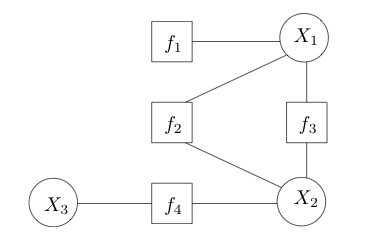
\includegraphics[width=0.4\linewidth]{./images/Factorgraph.jpg}
      \caption{A simple factor graph \cite{hwymeers_example_2008}.}
      \label{fig:ex_factor_graph}
    \end{figure}

      Designed for the FIRST Robotics Challenge, frameworks such as Sensor Fusion 2 (SF2) provide users with algorithms for an integrated platform. Some examples are latency correction between IMU and camera data, fusion of encoder and IMU data, and keyframe-based state estimation \cite{kauai_labs_inc_video_2017}. Again, these algorithms use known system parameters, such as update frequencies of sensors, frame transformations between sensors, and data from landmarks for filtering and position estimation. Usually, the IMU data is available at a rate an order of magnitude larger than that of the camera. Additionally, the data is accurately timestamped and easily accessible to the vision processing thread. This way, the user receives an updated pose estimate without lag and has a history of the orientation. This is useful for trajectory planning or on-line path correction (like recovering from a collision). Within the next several years, systems like this will mature, offering localization or possibly SLAM.

  \subsection{Beacon systems and Wireless Networks}

    Beacon systems have been used many times with success in the literature. Generally, these systems use ultrasound and or radio as a medium and either signal strength, phase shift, or time to measure distance to the beacons. Among radio systems, the system in \cite{bahl_radar:_2000} identified the location of people moving around buildings using signal strength in the 2.4gHz band received at three or more beacons, and they report accuracy of a few meters with an update rate of at most four times per second. The systems described in \cite{digiampaolo_mobile_2014} uses passive RFID tags on the ceiling and an RFID transmitter on the robot, and report an accuracy of 4\si{\centi\meter} within a 5\si{\square\meter}. Another RFID system \cite{saab_standalone_2011} also uses signal strength to RFID, and reports accuracies for various configurations ranging from 1\si{\centi\meter} to 3\si{\meter}. These RFID systems use readers that cost over \$500.

    There are also countless localization systems that use standard wireless networks. A comprehensive survey of these systems can be found in \cite{liu_survey_2007}. Systems that use signal strength in standard wireless LAN networks have achieved up to 10\si{\centi\meter} accuracy and hundreds of updates per second. Another radio beacon solution is to substitute single-frequency radio with Ultra-wideband radio. These systems can achieve centimeter level accuracy, but they use obscure or custom made transmitters and receivers that cost in the hundreds of dollars \cite{zebra_dart_2017} \cite{pozyx_pozyx_2017}.

    Among ultrasonic beacon systems, \cite{kleeman_optimal_1992} uses the raw arrival times of ultrasonic pulses over time plus odometry together in a Kalman filter. Many beacon systems use the speed difference between sound and electromagnetic waves to measure system. Systems like \cite{smith_tracking_2004}, \cite{ward_new_1997}, and \cite{kim_advanced_2008} send radio pulses followed by ultrasonic pulses. Nodes in the network us the difference in arrival time of these two signals to measure distance. Alternately, some systems use infrared pulses in place of radio \cite{ghidary_new_1999} \cite{yucel_development_2012}. These systems are inexpensive, and report accuracy of between \SI{2}{\centi\meter} and \SI{14}{\centi\meter}.

  \subsection{Cameras with Visual Tags}

		Vision based localization is widely used in robotics. Different visual approaches have been applied to mobile robot systems. Most of vision based systems have cameras on the robots and had either natural landmarks or artificial landmarks in the environments as references to absolute positions. If the natural landmark approach is used, knowing the absolute positions of objects in the circumstance, a robot could calculate its absolute position by calculating orientation and distance toward the object detected and recognized with its absolute position. Another similar approach is using 3D models and 2D to 3D matching techniques. The system described in \cite{sattler_fast_2011} had accurately localized the camera's position using this 2D to 3D mapping technique. Among all of the vision based approaches, the usage of a combination of cameras and artificial landmarks to localize robots is one of the most popular. Common artificial landmarks include 1D binary barcode, 2D binary barcode and 2D colored barcode. The system in \cite{lin_localization_2004} applied the approach of using cameras and ID tags. The system had ID tags on the ceiling, which were \SI{2}{\meter} away from the floor. A web camera, facing to the ceiling, was mounted on a moving robot with a speed of \SI{20}{\centi\meter\per\second}. This system measured the position and orientation of the robot relative to the ID tags through image processing. The result of the experiment in \cite{lin_localization_2004} showed that this method was accurate even though there was an unevenness between the ceiling and the floor. Another system \cite{huh_mobile_2007} also used camera and tags. However, instead of sticking ID tags on the ceiling, it put invisible tags on the floor by every \SI{3.75}{\centi\meter}. The camera it used was surrounded by a UV light, which allowed the camera to capture those invisible tags. This system performed really well in homelike environments, it only had few centimeters of error. Another barcode based localization system of low capacity mobile robot (8 KB memory, 16 MIPs) \cite{dias_barcode-based_2012} used 1d barcodes as references. Using a camera with 80 vertical pixels and 640 horizontal pixels, the system achieved localization within \SI{3.5}{\meter\per\second\square} of error on average. An experiment on 2D barcode based localization was performed on a Pioneer 3 - AT robot. The robot was placed in a random location in the environment and had a Canon VC-C50i analog camera connected with a \SI{1.8}{\giga\hertz} processor and worked under Linux operating System. The robot moved with a speed of \SI{50}{\milli\meter\per\second}, trying to locate itself by finding a code vertically mounted on a wall. The code contained information about its xyz position, normal vectors and its length, therefore, the system would not need to query through databases to find information, which made the process faster.

	\subsubsection{ArUco and MarkerMapper}

    The ArUco library provides a function for estimating the pose of an object by minimizing the squared sums of the distances between the projected points and the measured points (reprojection error). The side length of each tag is known and input into the program. The measured points (two corners, minimally) are used to obtain a point estimate in 3D space. Multiple point estimates from each corner are used to calculate the pose of the ArUco tag's centroid. The projected points are described by the camera matrix, which is a model for a pinhole camera discussed above. The reprojection error corrects the pose estimate based on the calibrated values.

    \begin{figure}[H]
      \centering
      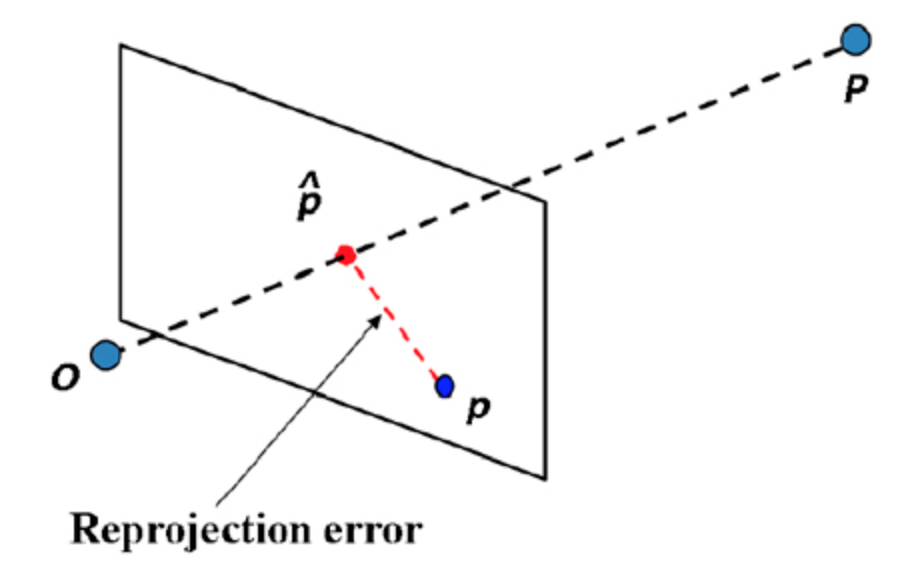
\includegraphics[width=0.5\linewidth]{./images/reprojection_img.png}
      \caption{Calculating reprojection error \cite{richard_hartley_multiple_2003}.}
      \label{fig:reprojection_img}
    \end{figure}

    The ID of the origin is input into the program. By estimating the pose of each tag in a camera frame, a map of transforms between tags was developed. The user must first map their work space by collecting transform data.

    \begin{equation} \label{eq:PoseDefCamera}
      p =
      \begin{bmatrix}
        t \\
        r \\
      \end{bmatrix}
      =
      \begin{bmatrix}
        t_x \\
        t_y \\
        t_z \\
        r_x \\
        r_y \\
        r_z \\
      \end{bmatrix}
    \end{equation}
    \begin{equation} \label{eq:TransCamera}
      T_0^1 = p_1 - p_0
    \end{equation}

    The map is complete when the user is able to query the pose from the origin using data from any tag in the workspace. Previous research indicates that calculating the transform between tags is sufficiently accurate. This protocol is preferred because it does not require the user to manually measure distances between tags and input them into the program. Instead, the user generates the map using the camera. Presently, the algorithm fails to utilize redundant information and instead computes position based on the first tag detected in the image. Future progress includes utilizing a least-squares solver for optimizing the pose estimate using information from all tags in a frame. Finally, to obtain the pose of the robot from the camera, the transform between the camera and the centroid of the robot must be computed.

    \begin{figure}[H]%
      \centering
      \subfloat[raw data]{{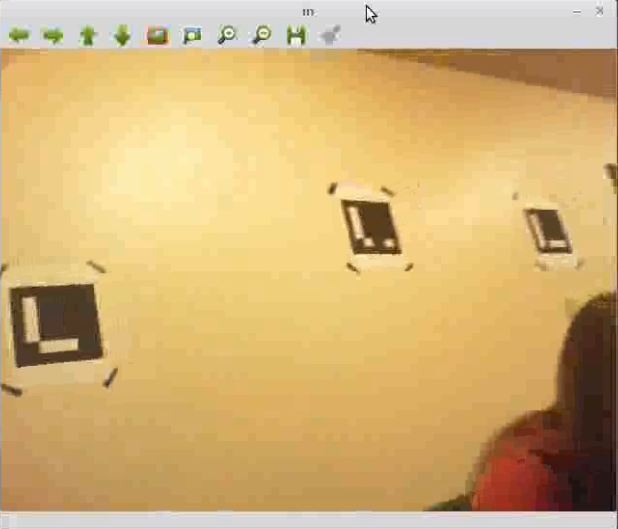
\includegraphics[width=5cm]{./images/aruco_vis2.png} }}%
      \qquad
      \subfloat[annotated frame]{{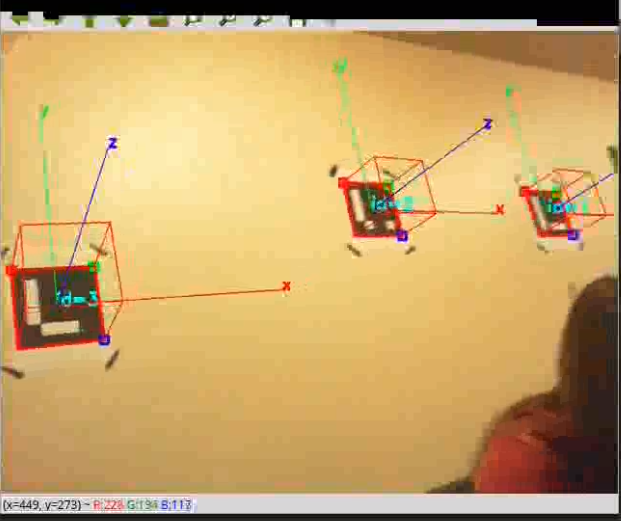
\includegraphics[width=5cm]{./images/aruco_vis1.png} }}%
      \caption{Visualization of pose estimate}%
      \label{fig:arucoVis}%
    \end{figure}

  \subsection{Optical Flow}

    Optical flow is the ability to track changes between cameras frames and measure the differences between them to track position. In other words, optical flow is where given a sequence of images it can find the movement of objects between the images. More exactly optical flow looks at the movement of pixels among images. There are many assumptions about the image that has to be made in order to calculate in order to calculate optical flow. The first is that the lighting in the image stays consistent throughout the sequence of images. Images with inconsistent lighting or transparent objects would violate this assumption. Limiting the amount of inconsistencies in each sequence of images leads to more accurate optical flow.

    There are many methods of calculating optical flow that deal with different constraints. This first is the Horn and Schunk method which calculates optical flow looking at all pixels in an image making it considered a global method. Along with the lighting constraint it also adds that the image should be as smooth as possible and have few variations in its coloration. The closer the amount of variations is to zero the more accurate the optical calculation will be\cite{odonovan_optical_2005}.

    The optical flow vector for each pixel is calculated using the equation below. $I_x$  and $I_y$  are the spatial gradient of the current pixel. Spatial gradients refer to the the path the pixel is moving along. $I_t$ is the temporal gradient of the current pixel. Temporal gradient is how similar the motion of the pixel is to its neighbors \cite{sun_optical_2008}. $\alpha$ is a weighting term. $\bar{u}$ and $\bar{v}$ are the components of the average optical flow vector of neighboring pixels. The equation is shown below \ref{eq:hotnandschunk} \cite{odonovan_optical_2005}. $n$ represents which iteration the optical flow calculation is on. Each current pixels optical flow is calculated based on previous iterations pixels. Optical flow calculation will iterate from pixel to pixel until it has calculated optical flow for each pixel.

    \begin{figure}[H]
      \centering
      \begin{equation}
        \begin{split}
          u^{n+1} &= \bar{u}^n-\frac{I_x[I_x\bar{u}^n+I_y\bar{v}^n+I_t]}{\alpha^2+I_x^2+I_y^2} \\
          v^{n+1} &= \bar{v}^n-\frac{I_x[I_y\bar{u}^n+I_y\bar{v}^n+I_t]}{\alpha^2+I_x^2+I_y^2}
        \end{split}
      \end{equation}
      \caption{Horn and Schunk Optical Flow vector equation}
      \label{eq:hotnandschunk}
    \end{figure}

    Optical flow can also be done locally using the Lucas Kanade method \cite{sun_optical_2008}. This method is based on the assumption that the optical flow vector of pixels are similar to their surrounding pixels. This method finds optical flow vectors that are consistent with its neighboring pixels' temporal gradients and spatial gradients. Each neighbor is then given a weight based off of how close it is to the pixel. The farther away a pixel is, the lower a weight it is assigned. This is because spatial and temporal gradients are based on how far away a pixel is so the error will be larger. Having a lower weight will reduce the error. The formula for the optical flow vector is a least squares equation shown below in equation \ref{eq:lucaskanade} \cite{odonovan_optical_2005}.

    \begin{figure}[H]
      \centering
      \begin{equation}
        \begin{split}
          E_v &= \sum_{p\in\Omega}W^2(p)[\nabla I(p)\cdot v + I_t(p)] \\
        \end{split}
      \end{equation}
      \caption{Lucas Kanade Optical Flow vector equation}
      \label{eq:lucaskanade}
    \end{figure}


    $\nabla I(p)$ and $I_t(p)$ are the spatial gradient and the temporal gradient for each of the neighboring pixels $p$. $v$ is the optical flow vector for pixel located at $(x, y)$ on the image. $W(p)$ is the weight assigned for each pixel. Local methods tend to work better since they do not allow information about vectors to spread to unrelated regions of the image. This issue of information spreading to unrelated areas of the image is especially problematic in global methods when the assumptions about consistent smoothness and illumination are not fully met. There are a variety of other optical flow methods that focus on different ways of comparing pixels within images but local and global are the most popular methods \cite{odonovan_optical_2005}.

    Lucas Kanade looks at pixels which have a large gradient in intensity of color. It changes images to be gray scaled in order to see changes in darkness instead of colors. Lucas Kanade method works the best when it uses pixels that have three qualities. The first is that the pixels in a small area have the same brightness. Even though the location of the pixel has changed the brightness is consistent, so using a pixel from that area to track is optimal. They also should be temporally similar meaning the path the pixel takes should change gradually. Pixels should also be spatially similar, meaning that neighboring pixels should have similar motion to each other. Picking pixels that fit these requirements work best with Lucas Kanade \cite{sun_optical_2008}.

    Optical flow has been used for multi-sensor localization in indoor, feature-rich environments \cite{gao_qingji_onboard_2015}. Using a PX4FLOW optical flow sensor, 64x64 pixel images were captured at 100 FPS, and an ultrasonic range sensor measured distance from the ground. The data from the camera was used to obtain a velocity information using optical flow and a position estimate using landmark detection on the images. These were fused with attitude data from an onboard IMU. In this research, miniature quad-copters flying over a textured carpet are used to evaluate the localization algorithm. The patterns on the 20x20m carpet, comprising dots of random size and a 1 square grid, are used as features for the optical flow and camera-based position estimates. The algorithm developed is benchmarked against results from an open-source optical flow position estimate provided with the sensor's API \cite{dominik_honegger_open_2013} and are compared qualitatively using the below plot.

    \begin{figure}[H]
      \centering
      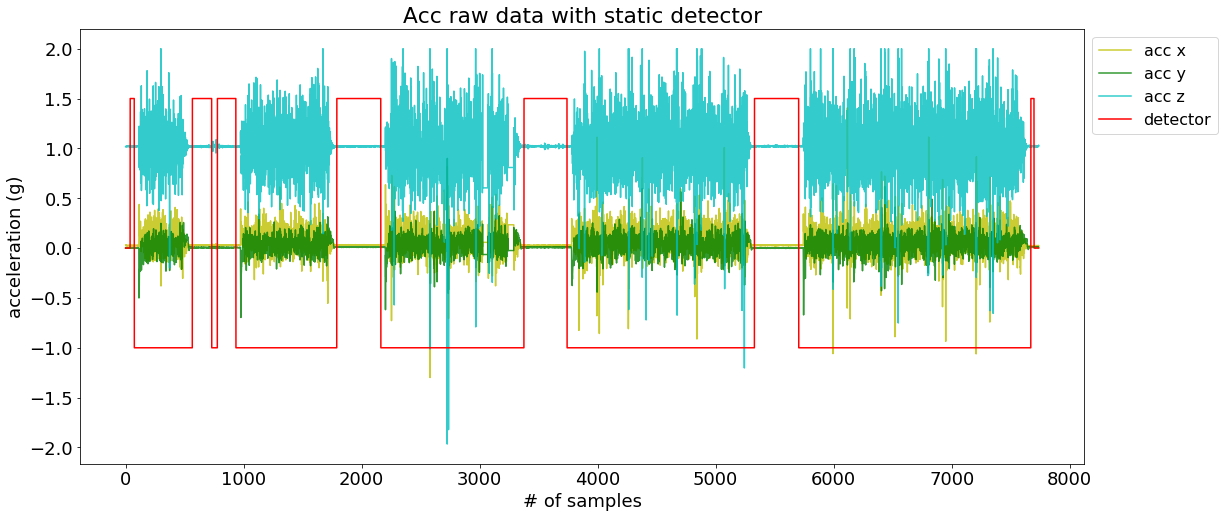
\includegraphics[width=1\linewidth]{./images/static_detector.png}
      \caption{This should be a plot of optical flow data compared to the algorithm developed by Qingji et al.}
      \label{fig:gao_qingji_onboard_2015_results}
    \end{figure}

  \subsection{Filtering and Calibration} \label{filtering}

    Given the number of sources of position information, it is natural that there will also be a number of ways to take advantage of using multiple techniques together. Different sensors can have better or worse performance in different scenarios, and a choice of fusion algorithm will yield more accurate position information by leveraging this. Calibration can also be used to compensate for errors between sensors. For instance, if your have encoders to determine that you are not moving, you can calibrate your IMU knowing this fact. The class of filtering algorithms we explore is called Bayesian filters. These filters describe the world and sensors with probability models, and they estimate both the state of the robot and the confidence of that state estimate. Bayesian filtering algorithms include Kalman filters, information filters, and particle filters. Kalman filters and information filters have the advantage in computational efficiency, where as particle filters can more be more accurate if the true belief distribution is non-gaussian or if the true dynamics are nonlinear \cite{thrun_probabilistic_2005}. In our work, it is natural to consider the state as the position, velocity, and acceleration of the robot. We claim that this state representation satisfies the Markov condition needed by Bayesian filters, which is that our current state is sufficient to make future predictions. To implement these filters, we required a model for now our state changes given our current state and motor inputs. For each measurement source, we define how the sensor values are derived from the state. It is easy to come up with very rough approximations for these equations, but difficult to construct accurate ones. On the other hand, these filters have very strong gaurantees and their efficacy has been demonstrated in numerous systems \cite{chui_kalman_1991}\cite{digiampaolo_mobile_2014}\cite{mirzaei_kalman_2008}\cite{nasa_kalman_1999}\cite{saab_standalone_2011}.

    Many of the localization techniques discussed involve some form of calibration. Primarily, the IMU requires calibration for misaligned axis, scaling factors, and biases. There are many procedures for calcuating these calibration parameters by taking advantage of static intervals and assumptions about the force of gravity \cite{lupton_visual-inertial-aided_2012}\cite{lee_test_2011}\cite{tedaldi_robust_2014}. Visual tag detection algorithms, such as ArUco, also include a camera calibration process to account for the focal length, field of view, and distortion characteristics of the camera \cite{itseez_calibration_2017}. Knowing these parameters allows one to undo distortion to the image, which is essential for detection of most AR tags.

\section{Trade-Off Analysis Of Different Techniques} \label{section:methods}

  Each of the techniques presented thus far have strengths and weaknesses. In cases where those strengths and weaknesses are orthogonal, combining multiple techniques improves the overall performance. This is the fundamental principle behind sensor fusion. For example, in \cite{kim_advanced_2008} the authors use a compass to make up for the inability of beacons to measure orientation of the robot. In order to tackle all of the diverse challenges of localization in the FRC environment, we believe it is necessary to combine techniques. In this section we will explain which techniques we have selected for our system and which we have ruled out. We will justify why none of the techniques discussed are sufficient on their own, and explain which the techniques we have chosen work well together.

  As stated in section \ref{section:related_work}, techniques for localization include LIDAR mapping, ultrasonic mapping, IMU and encoders, infrared or radio and ultrasonic beacons, wireless network methods, cameras with tags, and optical flow. Each of these techniques has been used successfully in their respective applications, but not all of them are appropriate for this project.

  LIDAR has been shown to be one of the highest performing localization methods in terms of accuracy, precision and update rate. The two reasons why we are not pursuing it further are because it is too expensive and because it requires a map. LIDARs capable of ranging across an entire FRC field are over \$400, which is the cost limit for any single part on an FRC robot. Additionally, LIDAR techniques also require either mapping on the fly, or an existing map. Mapping on the fly presents its own challenges, and usually suffers from very bad localization for some initial period of time while the map is built. Therefore, a map would have to be provided for the environment. Existing maps would work very well on the competition FRC fields, but would not apply in the practice spaces teams us, and it is unrealistic to have a consistent practice space in an FRC shop.

  Ultrasonic mapping has this same issue. Both LIDAR and ultrasonic mapping would work best if teams to place walls up to create a ``pen'' for the robot of known geometry to use as a map, and for this reason we believe LIDAR and ultrasonic mapping are unfit. Another major issue with ultrasonic mapping is the interference between robots. If multiple robots range ultrasonic near one another, there could be cross talk or interference between the signals. This is reason enough to rule out any use of reflecting ultrasonic. Note however that ultrasonic beacons do not have this weakness, since the pulses being emitted are not expected to reflect.

  IMUs within the budget of FRC teams suffer from accumulated drift, and as such they cannot be used in isolation. On the other hand, many FRC students have experience with them, so it would be wise to support basic features such as heading detection and filtering using IMUs. IMUs also complete other localization techniques very well. For example, cameras suffer from the jitter of the robot moving, and encoders fail when the wheels slip. IMUs on the other hand are excellent at detecting jitter and slippage. In this way, an IMU is a good complement to cameras and encoders.

  Radio and ultrasonic beacons are very attractive because of their low cost and ability to automatically locate each other. The cost of each beacon, according to the specifications laid out in section \ref{section:system_spec}, are projected to cost about \$30 (see \ref{table:beacon_bom}). Furthermore, beacons have more flexibility in their placement than tags because they are much smaller and do not need to be on flat surfaces, or in specific orientations. Finally, because each beacon can operate as a transmitter or a receiver, beacons can automatically locate each other which means students will not have to measure their positions or worry about them moving. A procedure for this self-localization is described in section \ref{section:beacon_self_localization}. Beacons also make up for some flaws in the other techniques. Beacons provide absolute global position but updates slowly, which nicely complements IMU and encoder methods which are fast but only measure changes in position. Additionally, beacons are more resistant to jitter than cameras. Finally, by placing the beacons and cameras in different locations we can minimize the effect of occlusion.

  Wireless network systems are among the most popular for indoor localization. However, they also require knowledge and control over the 2.5 gHz spectrum in the area where they are used. At FRC events, there can be dozens of wireless networks running, as well as the wireless networks used on the field for communication between robots. For this reason, we feel that techniques using wireless frequency have too many unknown variables.

  Among the vision based localization systems discussed in the Literature review, there are systems that use natural landmarks (object detection) and those that use artificial landmarks (tags). Tag based systems are preferred because they are inexpensive and easy to implement. Natural landmark detection would not perform well because the field of FRC changes over time and the robots are moving around the field during the competition. Furthermore, implementing real time object recognition is computationally intensive. Among systems using artificial landmarks, not a lot of robot localization systems use 1D barcodes as references. A 1D barcode can only contains up to 25 characters, which limits the length of information. Among 2D barcodes, fiducial tags and QR tags are two of most popular choices in mobile robot localization. The advantages and disadvantages of different types (QR, Data matrix, PDF417, fiducial tag) of 2D barcodes are discussed here. QR codes are designed to align with the camera. It contains 268 pixels without payloads. Data Matrix codes are very similar to QR codes, and they have high fault tolerance and fast readability. Data Matrix can be recognized with up to 60\% of the code unrecognizable. PDF417 is famous for a storage of huge amount of data. Complex information such as photographs, signatures can be inserted into PDF417 easily. Fiducial tags contain less information than QR codes. However, many of them can easily be detected in one shot and the process speed for fiducial tags is faster than of QR codes. One of the most commonly used 2D barcode in robotics is fiducial tag. A system in \cite{wang_apriltag_2016} measured the distance between AprilTags and the camera. A sheet of \SI{16.7}{\centi\meter} AprilTags were tested from \SI {0.5}{\meter} to \SI{7}{\meter} away. The calculated distance was almost the same as the real distance from \SI{0.5}{\meter} to \SI{6.5}{\meter}. The position errors were within \SI{0.1}{\meter} from range 0 to \SI{10}{\meter}. However, orientation errors were pretty high (\ang{1.5} off) when the off - axis angle was small, but were within 1 degree from \ang{20} to \ang{75} of off - axis angle. The detected rates for tags were 100\% from 0 to \SI{17}{\meter} away. This system showed that the combination of camera and fiducial tags can potentially localize robots accurately and precisely. The research, \cite{chen_two-stage_2013} developed an algorithm to enhance the quality of QR codes captured in order to improve the recognition rate. Its algorithm successfully recognized 96\% of QR codes under a variety of qualities captured by a mobile phone camera. The average time for decoding a QR code is \SI{593}{\milli\second}. Another deblurring method in \cite{xu_2d_2011} can be applied to enhance the quality of motion-blurred ArUco code.
  Another benefit of cameras with tags is that they provide global position information without much setup or infrastructure. However, camera based systems suffer from occlusion and jitter. They are also generally computationally intensive. These disadvantages can be mitigated with our other localization techniques. In summary, tag based camera systems have been shown to be very accurate and we will incorporate them into our system.
  Published by the developers of the ArUco tag detection and pose estimation algorithm, Marker Mapper is localization technique for indoor robots. Motion capture data suggests that it is comparable to sophisticated localization algorithms such as ORB-SLAM and LSD-SLAM\cite{munoz-salinas_rafael_mapping_2016}.
  \begin{figure}[H]
  	\centering
    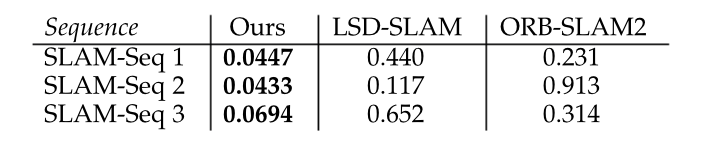
\includegraphics[width=1\linewidth]{./images/mm_errors.png}
    \caption{Marker Mapper absolute trajectory error (meters)}
    \label{fig:mmResults}
  \end{figure}

  The algorithm must first construct a map using off-line data. Once the transforms between tags are known, the map is used to report position from a known tag. The transforms between tags are corrected using redundant information in frames. The error along each basis cycle is computed, then an optimization algorithm is used to compute the corrected pose estimation. The mapping phase is an order of magnitude faster than Structure from Motion (SFM) and Multiple View Geometry (MVG) localization techniques. Although the paper mentions no on-line tests, is it reasonable to believe that pose estimation can be accomplished at minimally a 1Hz rate.

  Optical flow offers accurate angle measurements and fast updates that are relative to our current position. Like all camera based solutions, the vibration of the robot will likely makes this technique difficult. However, cameras are the most widely used sensor according to our survey of FRC students and alumni, which is another benefit of optical flow and tag based solutions. Optical flow can be applied either to cameras facing the environment or pointed down at the floor.
  The latter is the method used by computer mice, which have optical flow chips designed for high speed motion. Optical flow chips are made for optical flow detection with a specific lenses and microprocessor to get position \cite{font_characterization_2011}. These types of chips are built into computer mice with lenses that work only when the mouse is against a flat surface at a specific height from the table. This would be a problem in FRC since the field is not perfectly flat and there are sometimes obstacles that the robots need to drive over. There are also different drive trains which can shift center of balance between sets of wheels which would also cause the mouse to be off the ground. One of the benefits of using a mouse would the fast update rate. Optical flow mice update at 2,000 to 6,469 frames per second according to the ADNS-3080 optical flow sensors specifications \cite{sun_optical_2008}. They process frames quickly and most teams have mice of some sort they could use. However, a drawback of optical flow mice is their inability to detect rotation. Built into the sensors on mice are ways to ignore rotation since computer users want translation of the mouse to be measure over rotation in order to navigate a computer screen. Lighting is also important to for the camera to be able to clearly pick up images so having a source of light illuminating around the optical flow mouse would also be necessary for teams in order to get the best results \cite{font_characterization_2011}.

  The other option for optical flow is to use a camera which can be facing in any direction. OpenCV provides libraries and sample programs for running dense optical flow and sparse optical flow. The Lucas-Kanade method of sparse optical flow finds the best points on a frame and tracks the motion of only those points by comparing it to the motion of the pixels around that point. It is assumed all pixels around a point will have similar motion. Dense optical flow tracks the motion of all of the points on frames. Dense optical flow takes longer since it is using all of the points on a frame but can be more accurate \cite{itseez_opencv_2017}. In general, optical flow is not sufficient on its own because it does not provide global position information. However, it nicely complements our other systems because it uses a sensor we already plan to use, and provides a source of local position updates not based on any assumptions about wheels or robot dynamics.

  Ultimately, we have identified IMUs, encoders, cameras with tags, beacons, and optical as promising techniques for localization in FRC. These techniques together provide redundant sources of both local and global pose estimates, and account for many of the challenges associated with localization for FRC. We believe that implementing each of these techniques and combining their results will produce a more robust localization than exploring any one of them in depth.

\section{Defining Successful Localization in FRC} \label{section:defining_success}

  Here we present our goals and the criteria our system must meet in order to be successful. Broadly, we consider the following factors to be those which are important to the success of our system.
  \begin{enumerate}
    \item \textbf{Accuracy}\\ How close our position estimates are to ground truth.
    \item \textbf{Precision}\\ How close repeated position estimates are to each other given the same ground truth.
    \item \textbf{Update Rate}\\ How quickly does our system provide position estimates.
    \item \textbf{Accessibility}\\ How affordable is our system, how difficult is it to make, and how easy is it for teams to use.
  \end{enumerate}

  This goal for our system are as follows:

  \begin{enumerate}
    \item \textbf{Accuracy} of $\pm$\SI{10}{\centi\meter} and $\pm$\ang{5}
    \item \textbf{Precision} of $\pm$\SI{5}{\centi\meter} and $\pm$\ang{2}
    \item \textbf{Update Rate} at \SI{20}{\milli\second}/50FPS, with global updates at \SI{100}{\milli\second}/10FPS
    \item \textbf{Accessibility} with cost under \$200 for teams.
  \end{enumerate}

  To come up with hard numbers for these criteria, we first performed a few simple calculations based on our knowledge of FRC. First, we consider what teams would want to use position information for, and decided that the applications requiring the most accuracy are shooting and autonomous pick of game pieces at known locations. Both of these require the position estimates to be close to the true position of the robot. From there, we estimate that most FRC shooting and pickup mechanisms will work within $\pm$\SI{10}{\centi\meter}. Next, we decided the application requiring the most precision would be path following. If position estimates are imprecise and jump around rapidly, smooth path following will be difficult. From our experience with path following, we estimated that $\pm$\SI{5}{\centi\meter} and  $\pm$\ang{2} would be sufficient. For update rate, we considered what the maximum distance a robot could move within a period and used that to decide what our update rate should be. The very fastest FRC robots move \SI{6}{\meter\per\second}, which at an update rate of every \SI{20}{\milli\second} is a distance of $0.02*6 =$ \SI{0.12}{\meter}. The rate of \SI{20}{\milli\second} is a realistic cycle time in FRC, and we feel \SI{12}{\centi\meter} is sufficient given the speed. For accessibility, we acknowledged that teams cannot spend more than \$400 on any part, and that most times source parts from websites AndyMark, Cross-the-road Electronics, and National Instruments among other suppliers. We are also conscious that many FRC teams have limited or cluttered spaces for testing their robots, and may be working in a shared space that must be clean and usable after their work sessions.

  Using all of these informal estimates as a starting point, we conducted a survey of FRC students, alumni, and mentors. We received 65 responses in total, and used the results of this survey to solidify our design criteria. The full response of this survey are presented in \nameref{appendix:survey}. In summary, the median for accuracy was \SI{10}{\centi\meter} in x,y and \ang{5} in yaw. Our survey did not include questions about precision and update rate, because they depend on what position is used for. Instead, we asked if students would try path planning if they had a localization system, which would back up our estimate of precision. Our survey indicated that 90\% of students would try to make the robot autonomously follow paths. Therefore, our precision estimated based on path planning as an application is supported by our survey. Update rate was not addressed in the survey because we didn't think FRC students would have informed opinions on this metric. Finally, we asked several questions about the accessibility requirements. A cost of under \$200 was deemed acceptable by 84.6\% of responses, and so we have made \$200 our goal for cost. Furthermore, we learned that the amount of space in teams shops varies from a 5 by 5 foot space up to several thousand square feet, but the median shop size is 775 $ft^2$, which one can imagine as a 25 by 30 ft space. In terms of access, about 76.5\% of teams could leave up tags or beacons, with the others stating that they must clean up everything because they work in a shared space such as a classroom. Lastly, we asked students what sensors they were familiar with. The most familiar sensors were cameras (90\%), followed by encoders (84.6\%), then IMUs (60\%). Therefore, it would be beneficial to incorporate cameras, encoders, and IMUs because teams are already familiar with them. However, in order to not place extra constraints on sourcing parts, we choose to ignore the constraint that our system meet the FRC-Legal or Off-The-Shelf requirements of FRC.

  Ultimately, we formulated design criteria based on our own experience with FRC and with localization, as well as by conducting a survey of the needs, experience, and opinions of FRC participants. These design criteria will help us pick which localization techniques to pursue as well as define the goals for our system.


\section{Experimental Results} \label{section:experiments}

  One of the key contributions of this MQP is an extensive set of empirical and theoretical results spanning many different localization techniques. This sections describes each of these experiments and explains how each test impacts the practical implementation of a complete localization system.

  \subsection{IMU Calibration} \label{section:imu_calibration}

    From an early experiment collecting data on a Turtlebot, we saw that double integrating the accelerometer readings would not be accurate. This was expected, because it is well known the double integration will amplify any inaccuracies in accelerometer data. Therefore, we replicated the IMU calibration procedure described in \cite{tedaldi_robust_2014}, which accounts for many sources of error without requiring expensive external equipment. This calibration method was relatively to perform, and could be performed by FRC students. This calibration method corrects the misalignment, scaling, and biases in both accelerometer and gyroscope. This is done by solving for accelerometer calibration values that make the magnitude of acceleration during static intervals closest to 1, and then by solving for gyroscope calibration values that make the integral of gyroscope measurements between static intervals match the change in orientation between static positions. First, the IMU needed to be placed statically for a period of $T_{init}$ seconds. Next, by calculating the variance of the accelerometer data collected during that initialization period, a threshold for a static interval detector could be determined by applying a constant multiplier. After the initial waiting period, the IMU needs to be rotated an arbitrary amount and left in that orientation for 1 to 4 seconds. Each IMU position during the ``flip and wait'' period has to be distinct for calibration to be accurate. The entire ``flip and wait'' process has to be repeated 36 to 50 times. After all data was collected, an optimization proecdure was ran first on the accelerometer data to solve for the calibration parameters for misalignment, scaling, and bias that make the norm of the acceleration closest to 1. Then, a similar method was used for gyroscope calibration based on the success of accelerometer calibration. The quality of calibration of gyroscope was entirely based on the quality of the accelerometer calibration.

    In our experiments, we used $T_{init}=50$, as was reported by the authors for a different IMU. The authors arrived at this number from a plot of Allen Variance--we did not reproduce this plot with our IMU. We waited \SI{4}{\second} during our static intervals, but found that using $T_{wait}=3$ was better in practice for detecting wide, clean, static intervals. This is possibly because a sometimes the IMU was not truly at rest for a full four seconds. In our early experiments, we found that failing to record enough \textit{distinct} static intervals would cause the optimization procedure to fail to converge. So, in order to get as many distinct positions as possible, a Helping-Hands was used to hold the IMU. We rotated the IMU 36 times in total, which was the minimum suggested number of static intervals in the original paper. The accelerometer data and gyroscope data in $x$, $y$, and $z$ axis were recording for the entire period. Using the threshold from initialization data and the full accelerometer data, the static detector successfully distinguished between static intervals and dynamic intervals. A demonstration of our static detector is shown in Figure \ref{fig:static_detector}.

    \begin{figure}[H]
      \centering
      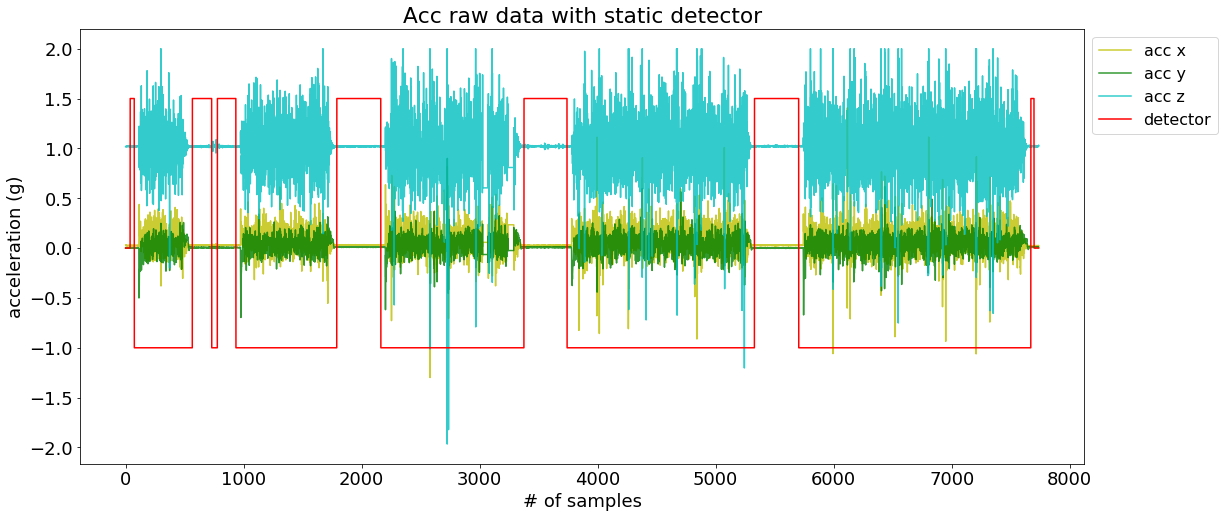
\includegraphics[width=1\linewidth]{./images/static_detector.png}
      \caption{The black line is 1 during intervals classified as static}
      \label{fig:static_detector}
    \end{figure}

    Using the identified static intervals, we optimize using the Levenburg-Marquedt procedure in python's NumPy package to solve for the accelerometer calibration values. The equation we are minimizing is shown below (Equation \ref{eq:accel_calibration_error}). These values can be found in Table \ref{table:imu_calibration_values}, and descriptions of each variable can be found in \cite{tedaldi_robust_2014}.

    \begin{equation} \label{eq:accel_calibration_error}
      \rVert g\lVert^2 - \rVert T^aK^a(a^s+b^a)\lVert^2
    \end{equation}

    \begin{table}[H]
      \centering
      \resizebox{\textwidth}{!}{
      \begin{tabular}{|c|c|c|c|c|c|c|c|c|}
        \hline
        $\alpha_{yz}$ & $\alpha_{zy}$ & $\alpha_{zx}$ & $s^a_x$ & $s^a_x$  & $s^a_z$ & $b^a_x$ & $b^a_y$ & $b^a_z$ \\
        \hline
        -0.002710 & 0.004559 & -0.000738 & 0.997279 & 0.996661 & 0.989960 & -0.006376 & -0.008999 & -0.019918 \\
        \hline
      \end{tabular}}
      \caption{IMU Calibration Values}
      \label{table:imu_calibration_values}
    \end{table}

    Note the values shown above are close to the values that represent no transformation, $[0, 0, 0, 1, 1, 1, 0, 0, 0]$. This indicates that our accelerometer is already quite well calibrated but not quite perfect, which is expected.

    The next step is to calibrate the gyroscope. We integrate the angular rates measured by the gyro between every sequential pair of static intervals and compare this to the angle between the two static intervals. We have a good estimate of the true orientation of each static interval from the previous accelerometer calibration step, and so the goal is to solve for gyroscope calibration parameters that make the integral of the transformed gyroscope data over the dynamic interval match the next orientation of the static interval as measured from the calibrated accelerometer readings. This is expressed in the error function we are minimizing, shown in Equation \ref{eq:gyro_calibration_error}.

    \begin{equation} \label{eq:gyro_calibration_error}
      \begin{split}
        % FIXME: this equation looks wrong
        \bigg\lVert u_{a,k} - \bigg(\int_{k-1}^{k} \Omega(\omega^S_i)di + u_{a,k-1}\bigg) \bigg\lVert \\
      \Omega(\omega^S_i) = T^gK^g(\omega^S_i+b^g)
      \end{split}
    \end{equation}

    The function $\Omega(\omega^S_i)$ takes the raw angular velocity readings $w^S_i$, transforms them with the calibration constants, and produces a rotation matrix. This rotation matrix is the euler rotation matrix (Roll-Pitch-Yaw ordering) which can then be multiplied by $u_a$. Towards this process, we investigated numerical methods for computing the above integral. This integral cannot be computed analytically because we only have samples of the integrad, rather than a analytic closed-form. Therefore, numerical integration methods like Euler's Forwardmethod or Runga-Kutta methods can be used. While \cite{tedaldi_robust_2014} uses Runga-Kutta 4th Order (RK4), we used the 1-step Euler's Forward method. Over the whole integral, this rotates the average acceleration values from the $k-1$th static interval, $u_{a,k-1}$, to the average acceleration values from the $k$th static interval. One could compute the same thing in a different order, by integrating the angular velocity values to get angles, constructing one rotation matrix, then rotating the acceleration values. However, because of gimble lock and dependence on ordering of the axis of rotation, this is much less accurate in practice. By rotating within the ingrand, we are only rotating by very small angles at a time, which mitagates the issues of using euler-angle rotation matrices. This theoretical result was tested experimentally, and the results are shown in Figure \ref{fig:gyro_integration}. Note that the bars representing the incremental rotation are more accurate than the one-shot rotation, where more-accurate is defined as closer to the true average acceleration readings at the next frame.

    \begin{figure}[H]
      \centering
      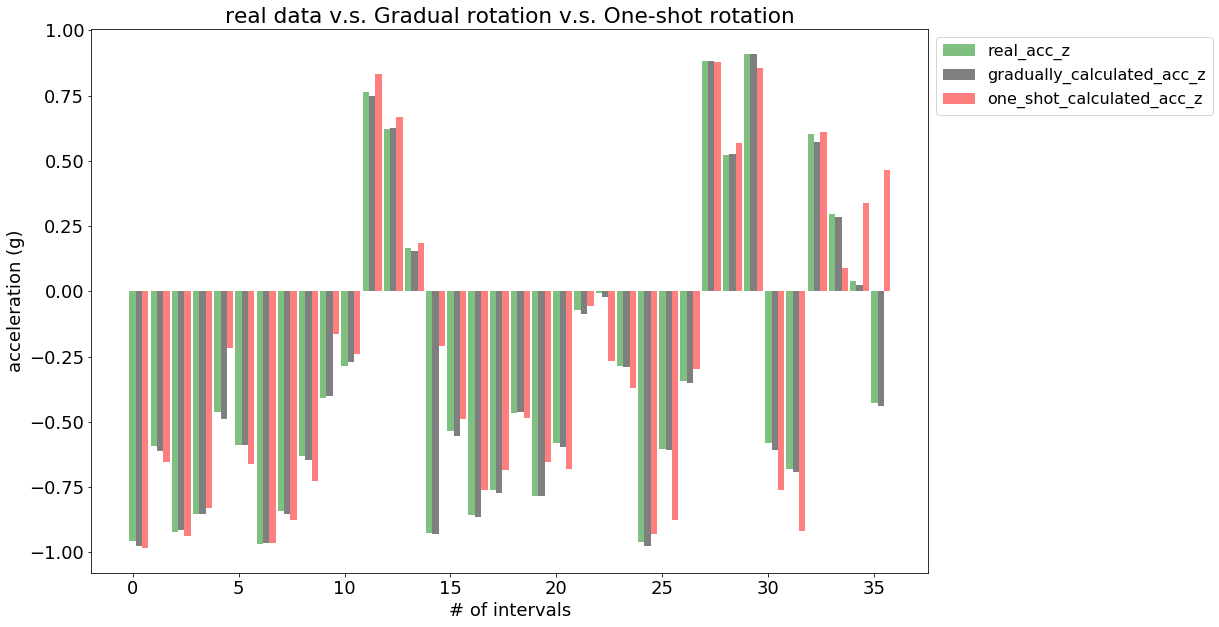
\includegraphics[width=1\linewidth]{./images/gyro_integration_y.png}
      \caption{Integration of the gyroscope readings in the Y Axis. Method 1 is one-shot rotation, Method 2 is incremental rotation. Incremental rotation is clearly more accurate.}
      \label{fig:gyro_integration}
    \end{figure}

  \subsection{Accuracy of Gyro Integration versus On-Chip Yaw Calculation}

    We asked the question of whether the provided on-chip \texttt{GetYaw()} method is more or less accurate than what can be computed from the raw gyroscope readings. To answer this question, we first used implemented a simple procedure for computing yaw from the gyroscope readings. First, we apply the calibration parameters (see section \ref{section:imu_calibration}), then a base-frame rotation. This base frame rotation accounts for the mounting of the NavX on our robot, which may not be perfectly flat. To do this, we let the robot sit still for a second or two and compute the rotation matrix that rotates the accelerometers readings to be $[0,0,1]$, which is the value you'd expect if the NavX were flat. Having calibrated and rotated the raw gyroscope readings in all axis, we can consider only the yaw or $z$ axis of the gyroscope. We use a 1-step forward Euler's method to integrate these readings, which are in degrees/second. This gives us our yaw angle over time.

    To compare this procedure with ground truth, we log the raw gyro values values while driving in the motion capture studio, then perform the calculations described above to get yaw. Figure \ref{fig:yaw_comparison} shows our computes yaw with the yaw reported by motion capture. Due to some strange wrap-around behavior, the mocap yaw has a small blip in value that can be safely ignored. Overall, our yaw value matches the ground truth very closely, with a maximum error of \ang{2.497} in the first 1000 samples (20 seconds).

    \begin{figure}[H]
      \centering
      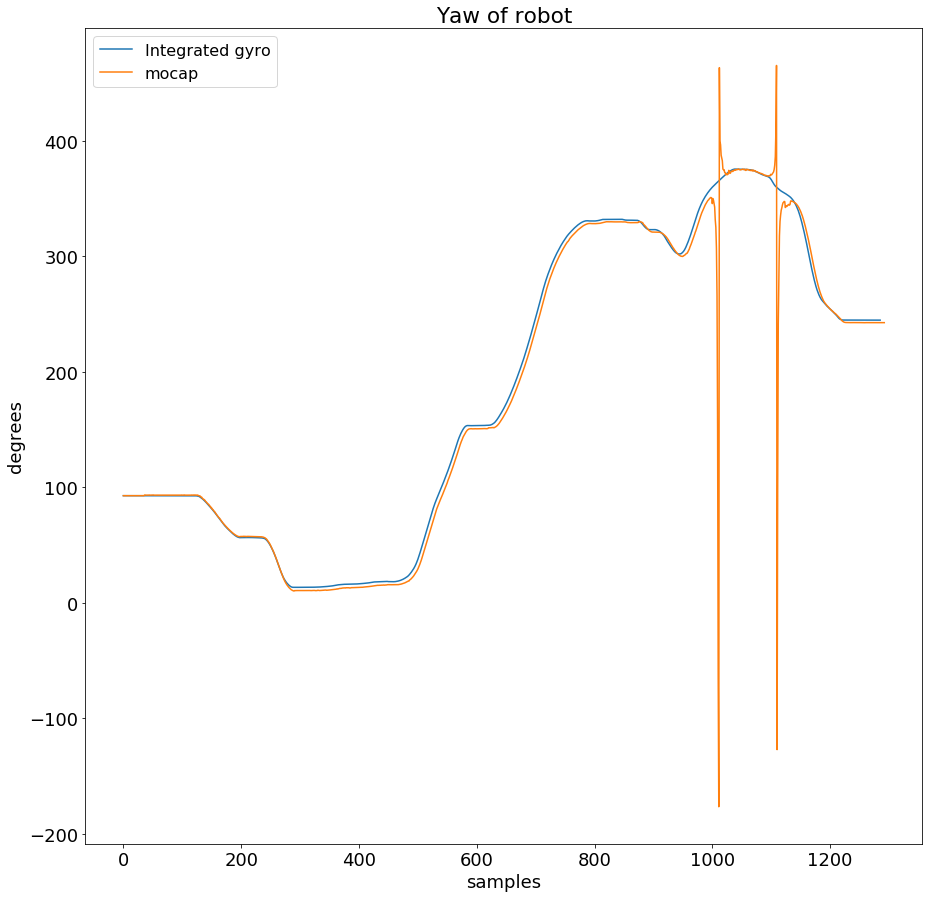
\includegraphics[width=0.75\linewidth]{./images/yaw_mocap_versus_integration.png}
      \caption{Comparison of yaw values between our algorithm and motion capture}
      \label{fig:yaw_comparison}
    \end{figure}

    Next, we compared the on-chip yaw to our integrated yaw method. %TODO: have some comparison between on chip and mocap or on chip and gyro integration

    % FIXME: log raw gyro during next mocap!

  \subsection{Characterising Drift and Bias in the Accelerometer}

    \subsubsection{Measuring the drift and bias in the accelerometer}

    % report the drifts and biases we saw in the circles test and in the
    % talk about how there weren't any obvious trends in bias
    % discuss the static tests you did where the rio was stationary, and report how much you say it drifting
    % we can do the same for the nypro stuff, showing how drift effects velociton and position as you integrate/double integrate

    \subsubsection{Drift Compensation}

    % then, explain what we tried to do to compensate for drift, and why it didn't really fix it

    \subsubsection{Zero Velocity Updates}
    % talk about how zero velocity udpates improve double integration/position

  \subsection{Comparing Our IMU Localization to the NavX API}

    % FIXME: how good is GetWorldX? Show mocap + nypro circles results
    % eventually also compare using with old/new mocap data

  \subsection{Measuring Beacon Delays}

    The beacon system relies on measuring the time it takes for a sound signal to travel from the beacons to the robot. To do this accurately, one must account for transmit and receive delays in addition to the actual time of flight. Figure \ref{fig:rx_tx_timing} illustrates the various delays we need to account for. We conducted experiments to estimate these delays. First, to get an estimate of the radio transmit and receive delay, a transmitter and receiver were set up on two microcontrollers. The transmitter sent \SI{5}{\milli\second} pulses at \SI{433}{\mega\hertz} (no encoded data) every \SI{55}{\milli\second}, and oscilloscope probes were attached to the input pin on the transmitter and the output pin on the receiver. By comparing the time difference between the input and output signals on the oscilloscope, we can determine the total time. Furthermore, we can measure the distance between the transmitter and receiver and subtract the theoretical time of flight from the total time. The full data for these measurements are available in \nameref{appendix:rf-rx-tx}, and an example measurement is shown in Figure \ref{fig:rf_delay_ex}. The time of flight of radio over distances of a new centimeters or meters is on the order of nanoseconds. We measured an average delay of \SI{45.175}{\micro\second}, which we attribute to the internal circuitry of the transmitter and receiver. The variance of this delay was \SI{16}{\micro\second}. However, we also measured delays as low as \SI{32}{\micro\second} and as high as \SI{79}{\micro\second}. Since the theoretical time of flight over the distances used in this experiment were at most \SI{1}{\nano\second}, we can conclude that there is both delay and significant variance in the delay of the transmitters and receivers. This is an important delay to consider when implementing the timing measurement of the beacon signals.

    \begin{figure}[H]
      \centering
      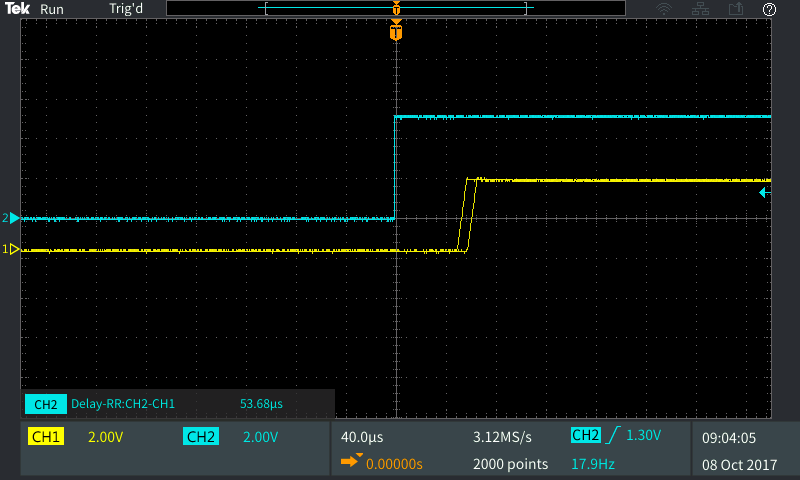
\includegraphics[scale=0.2]{./images/rf_delay_ex.PNG}
      \caption{Example measurement total trip time for radio signal. The blue line is the input to the transmitter, and the yellow are the output of the receiver}
      \label{fig:rf_delay_ex}
    \end{figure}

    Next we performed a similar experiment with the ultrasonic transducers. For this experiment, we used two NTX-1004PZ piezo speakers placed \SI{25}{\centi\meter} apart. The NTX-1004PZ is meant to be a high-frequency speaker for DJ equipment, and is designed to operate between \SI{4}{\kilo\hertz} and \SI{20}{\kilo\hertz}. However, because they are incredibly cheap we decided to evaluate them as ultrasonic speakers running just above that range. One was connected to a PSoC 5LP for transmitting, and the other was connected only to the oscilloscope. The other oscilloscope probe was connected to the transmitting piezo. The time difference between the transmitting signal and the receiving signal was measured. The signal applied to the transmitter was short bursts of a 24Hz square wave. Again, the distance was measured between the transmitted and received waveform, and the theoretical time of flight was subtracted. The full data for this experiment is shown in table \ref{table:us_delay}.

    \begin{table}[H]
      \centering
      \begin{tabular}{|c|c|c|c|}\hline
        Distance (m) & Expected Delay (us) & Measured Delay (us) & Error (Measured - Expected) \\ \hline
        0.10 & 294 &  390 &  96 \\ \hline
        0.15 & 441 &  556 & 115 \\ \hline
        0.20 & 588 &  698 & 110 \\ \hline
        0.25 & 735 &  872 & 137 \\ \hline
        0.30 & 882 & 1001 & 119 \\ \hline
      \end{tabular}
      \caption{Measured Delays in 2kHz Sine Wave Signal}
      \label{table:us_delay}
    \end{table}

    This data suggests that there is a constant delay of $\approx$\SI{115}{\second}, which could be attributed to the internal amplification circuitry and the time for the receiving piezo to begin to resonate. An example of the oscilloscope readings is shown in Figure \ref{fig:us_delay_scope}, which illustrates the time period where the receiving piezo response is building up before becoming detectable.

    \begin{figure}[H]
      \centering
      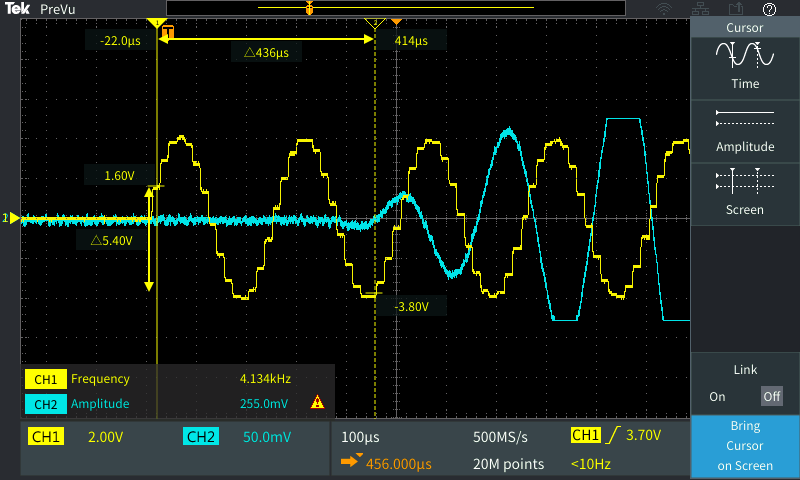
\includegraphics[width=0.8\linewidth]{./images/us_delay_scope.png}
      \caption{Capture of the measurement of ultrasonic delay on the oscilloscope}
      \label{fig:us_delay_scope}
    \end{figure}

  \subsection{Measuring Frequency Response} \label{section:frequency_response}

    After testing for delays, we also measured the frequency response of the NTX-1004PZ piezo speaker. We placed two speakers 17 feet apart, and using a function generator we transmitted a square wave at 8vPP and swept from \SI{20}{\kilo\hertz} to \SI{30}{\kilo\hertz} and back down over the course of 20 seconds. We attached an oscilloscope to the receiving speaker and captured the power at each frequency using the FFT mode, persisting the display over the course of the sweep to see how the frequency response changes across our frequency range. Figure \ref{fig:frequency_response} shows the results of this experiment. From this experiment, we learned that the best frequency response is achieved at \SI{22}{\kilo\hertz}, and the after \SI{27}{\kilo\hertz} the signal is indistinguishable from the noise.

    \begin{figure}[H]
      \centering
      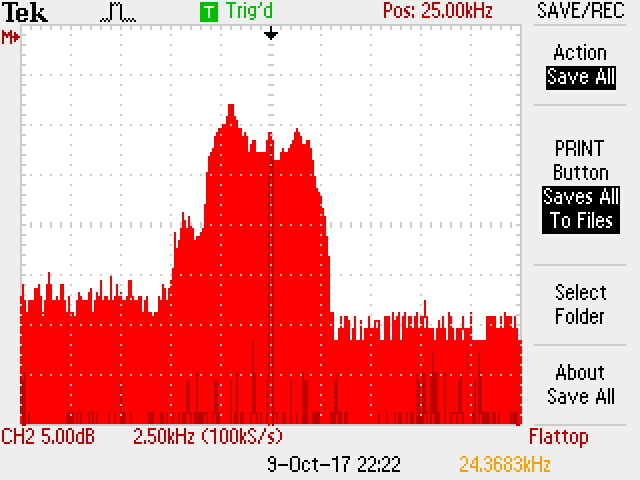
\includegraphics[width=0.7\linewidth]{./images/frequency_response.JPG}
      \caption{Frequency response of the NTX-1004PZ, centered at \SI{25}{\kilo\hertz} with \SI{2.5}{\kilo\hertz} per division. The best response is achieved at \SI{23}{\kilo\hertz}, and the highest detectable frequency is \SI{27.5}{\kilo\hertz}.}
      \label{fig:frequency_response}
    \end{figure}

    This experiment shows that any ultrasonic signals emitted by the beacons must be within the 20-27\SI{}{\kilo\hertz} range. For fixed frequency signals, \SI{22}{\kilo\hertz} should be used. Lower frequencies will be detectable and painful or annoying to humans, and higher frequencies will be undetectable.

	\subsection{OpenCV Optical Flow Sample Code}

    Preliminary testing with optical flow was done using a Microsoft USB camera using the sample code provided in OpenCV. In the screenshot below the window labeled flow that there are a variety of green dots on the screen. These are the points that dense optical flow has identified. There is also a green line which is the motion vector of which way the frames are moving. The middle window labeled HSV flow is adding color to the different points that are currently the best for tracking on the frame. The bottom window labeled glitch is the current frame and previous ones overlaid showing all of the motion that has happened.

    \begin{figure}[H]
      \centering
      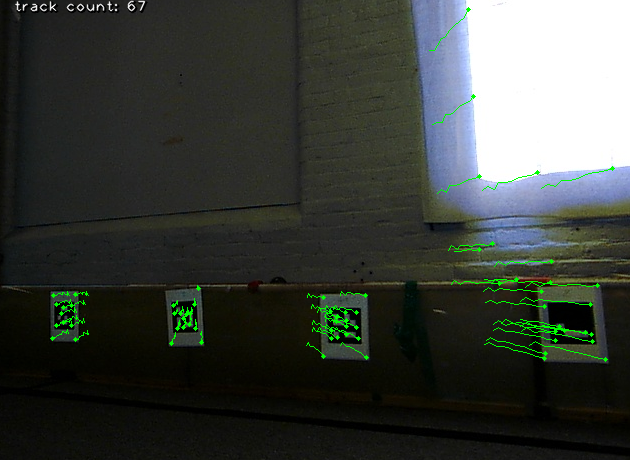
\includegraphics[width=0.49\linewidth]{./images/optflow.png}
      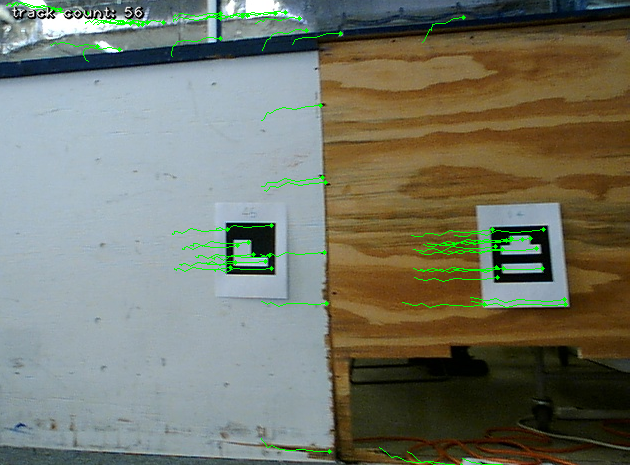
\includegraphics[width=0.49\linewidth]{./images/optflow_2.png}
      \caption{Screenshot of the opencv sample program \texttt{lk\_track.py} on video collected on a practice FRC field. Aruco tags provide excellent targets for Lucas-Kanade tracking.}
      \label{fig:opt_flow}
    \end{figure}

  \subsection{Benchmarking OpenCV Processing Times}

    This test compares computation time for optical flow with OpenCV. Tests were done using \texttt{lkdemo.cpp} which was we modified from a sample file provided by OpenCV. We compare this program on a laptop verse the RoboRIO and compare the time they took to run the code. The laptop used has a 2.8 GHz Intel 4 Core i7 processor. A chart below was made of the time that each program took to run 100 frames in seconds.

    \begin{table}[H]
      \centering
      \begin{tabular}{l|l|l|}
        \cline{2-3}
        & Laptop (sec) & RoboRIO (sec) \\
        \cline{2-3}
        & 3.638 & 8.429 \\
        & 4.184 & 8.429\\
        & 3.638 & 8.429 \\
        & 3.639 & 8.429 \\
        & 4.184 & 8.429 \\
        \hline
        \multicolumn{1}{|l|}{Average (sec)} & 3.8566 & 8.429 \\
        \multicolumn{1}{|l|}{Average (FPS)} & 26 & 12 \\
        \hline
      \end{tabular}
      \caption{Time for 100 frames to run using OpenCV on laptop verse RoboRIO}
      \label{table:optical_flow_benchmark}
    \end{table}

    We performed these measurements 5 times to check for repeatability. From these numbers, we conclude the laptop was just over twice as fast that of the RoboRIO. However, the 12 FPS rate is still fast enough for our project requirements (see Section \ref{section:design_criteria})

  \subsection{Collecting Ground-Truth with VICON Motion Capture}

    To evaluate the accurate of our system and to help with tuning various constants in the system we need a source of ground-truth state information. The ground truth data for measuring accuracy and precision is obtained using a VICON brand Motion Capture system. This comprises a VICON Lock+ data processor and 8 Vero infrared cameras. Our system can collect 2.2 megapixels of data and is designed for capturing human motion in small spaces. In our experiments, the space used for experimentation was 19x14 feet. The pose of the robot is tracked using three retro-reflective markers. These are positioned at known distances such that the transform between the centroid of the markers and the centroid of the robot is easily obtained. A scalene triangle laser cut from acrylic was used as a guide.

    \begin{figure}[H]%
        \centering
        \subfloat[guide for placement]{{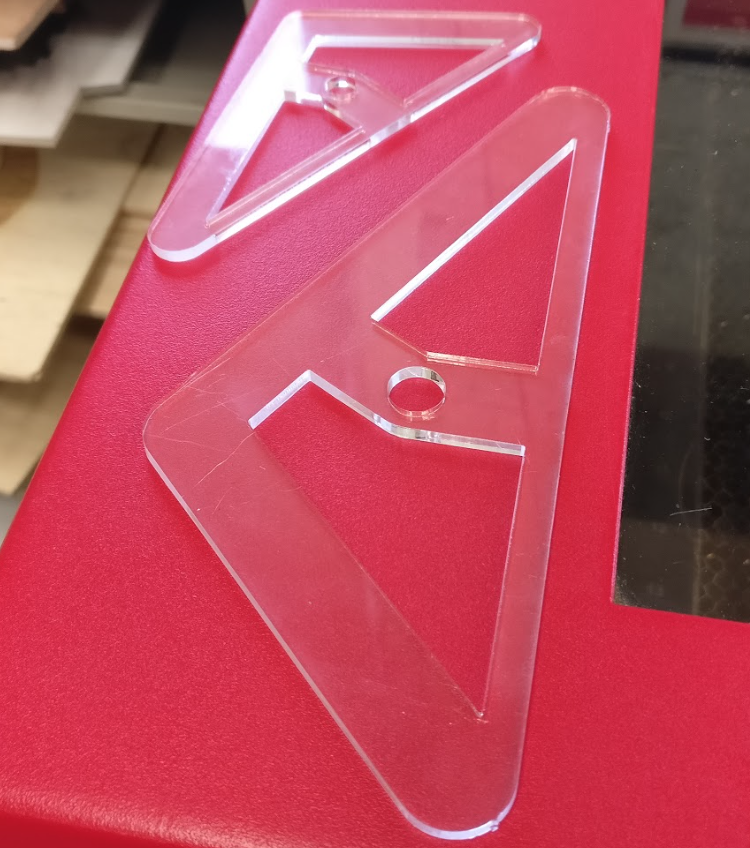
\includegraphics[width=5cm]{./images/calib_triangle.png} }}%
        \qquad
        \subfloat[reflective markers]{{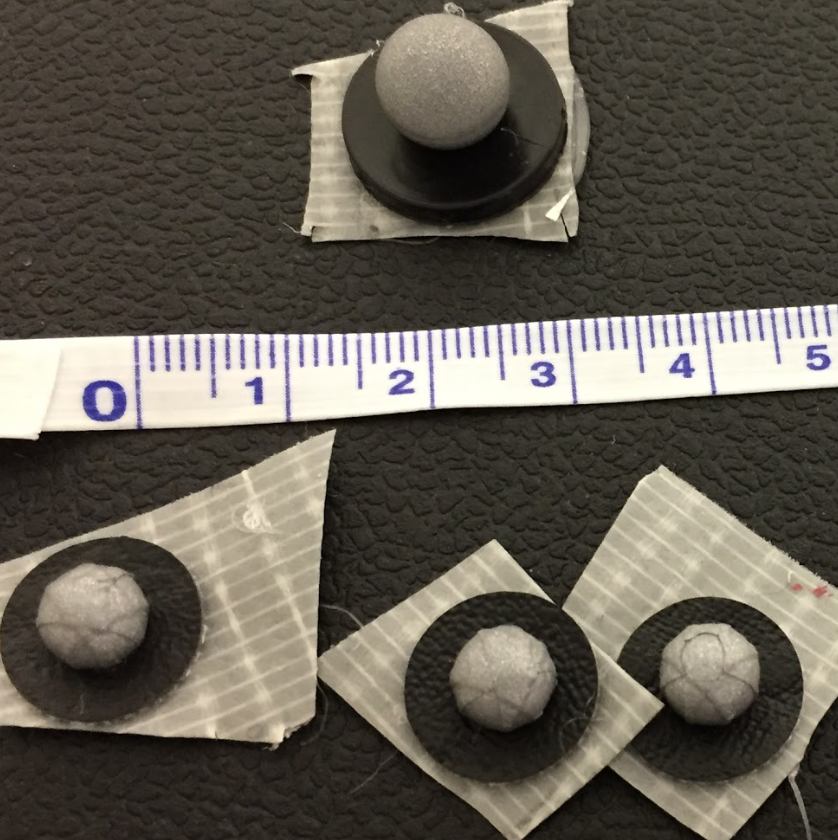
\includegraphics[width=5cm]{./images/vicon_markers.png} }}%
        \caption{VICON tracker set up}%
        \label{fig:viconSetup}%
    \end{figure}

    In our experiments, the camera system captures data at 100Hz. To synchronize data collection, the RoboRIO sends a 5V signal to the Lock+ processor, and a UDP packet is transmitted to the Co-Processor running the camera. This data is synchronous to within $\approx$\SI{500}{\micro\second}. Using the same markers, the pose of the ArUco tags is also measured.

    \begin{figure}[H]%
      \centering
      \subfloat[robot in VICON field]{{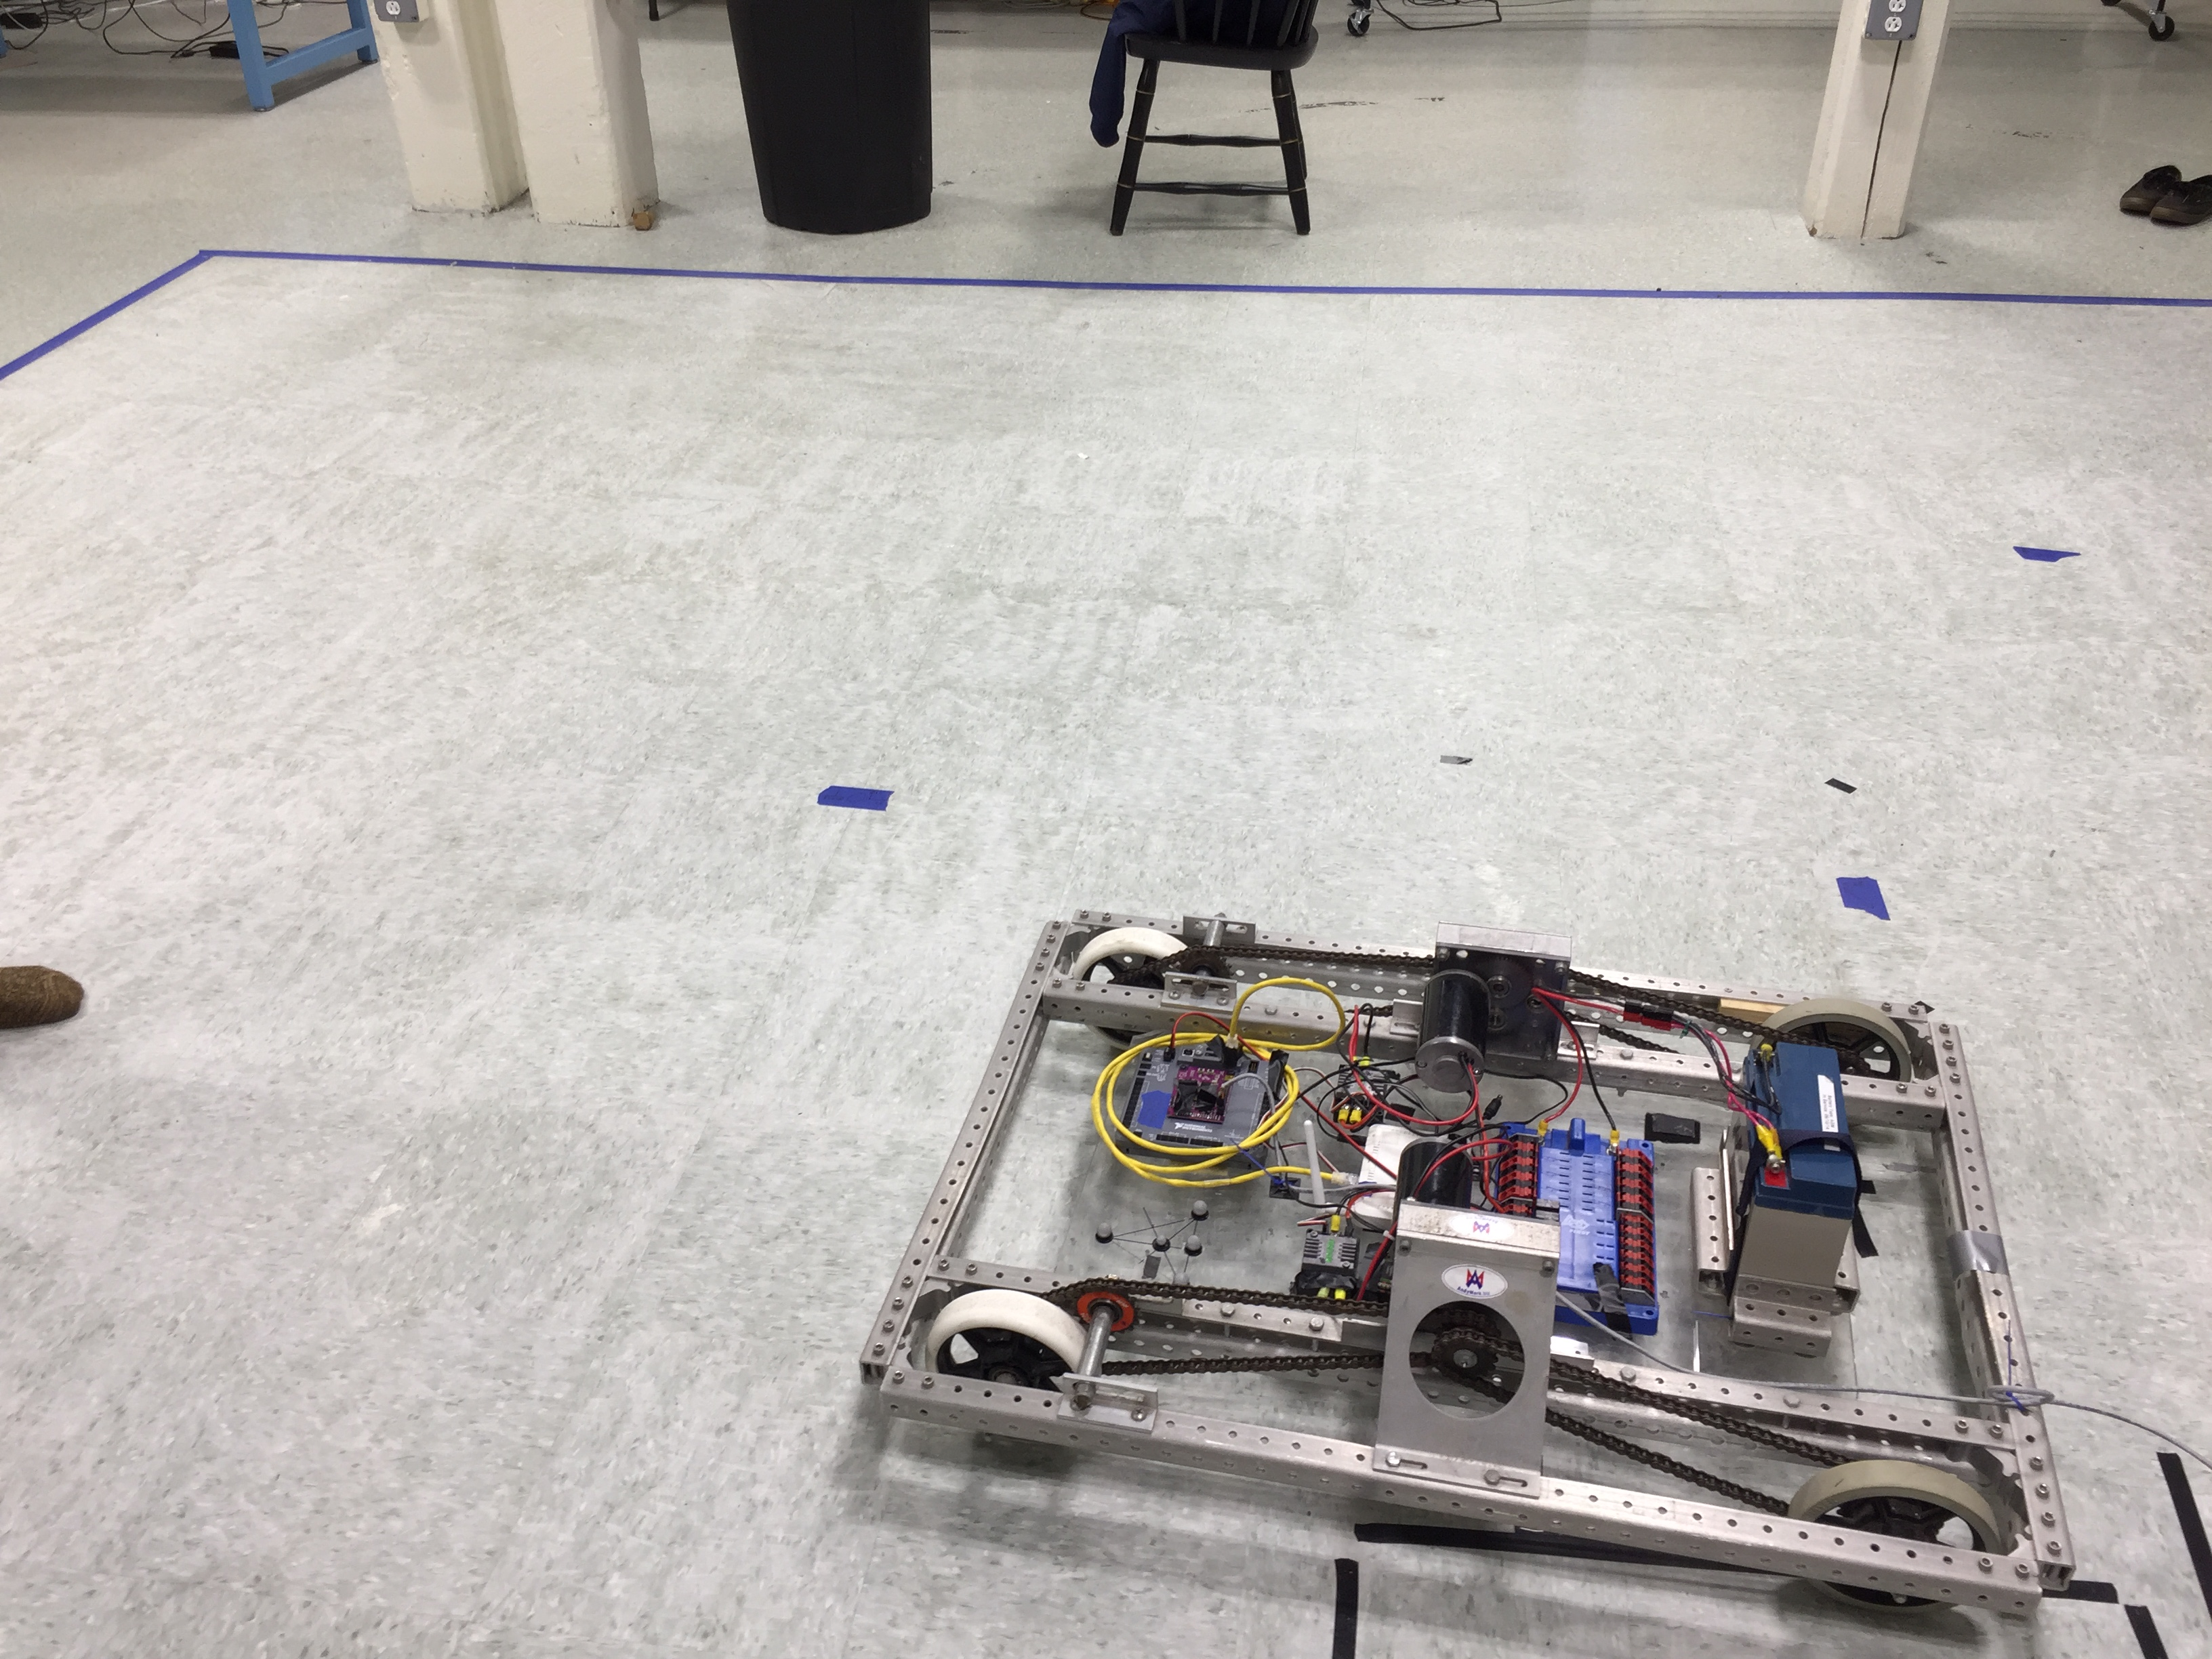
\includegraphics[width=5cm]{./images/robot_in_plane.jpeg} }}%
      \qquad
      \subfloat[IMU, encoder, and VICON position data]{{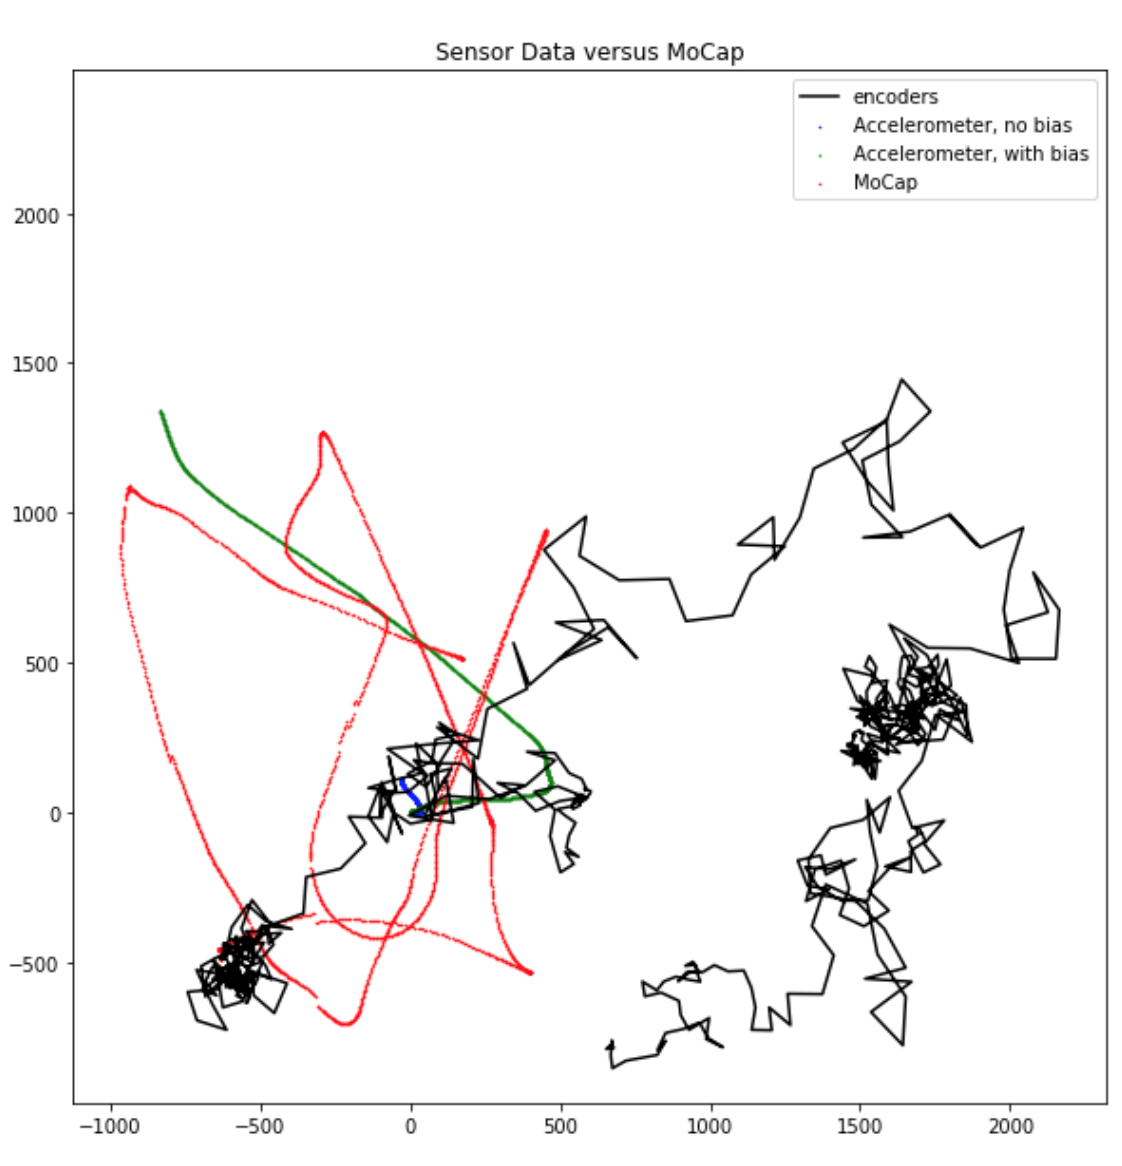
\includegraphics[width=5cm]{./images/imu_enc_vicon_data.png} }}%
      \caption{Collecting and Plotting Position data}%
      \label{fig:positionData}%
    \end{figure}

    % FIXME redo the results and change out the pictures above now that we have better results

  \subsection{Localizing with IMU and Encoder on the Turtlebot}

    % Describe Kacper's test with the Turtlebot under mocap

  \subsection{Detecting Simulated Chirps in MATLAB}

    In order to examine the theoretical limits of our ultrasonic chirp detection, we created synthetic chirps and examine how pattern matching filters would work to detect them. For our beacons to work we must be able to very precisely find the start of a chirp given a buffer of ADC readings, and we simulate this in MATLAB. In these experiments, we construct our chirps using matlab's \texttt{chirp} function, and we sweep from 20-27\SI{}{\kilo\hertz} (see section \ref{section:frequency_response} for justification). This signal is shown in figure \ref{fig:unshifted_no_noise_chirp}. The zoomed in version highlights that given a reasonable ADC speed of 108ksps, we will only see a very rough sine wave.

    \begin{figure}[H]
      \centering
      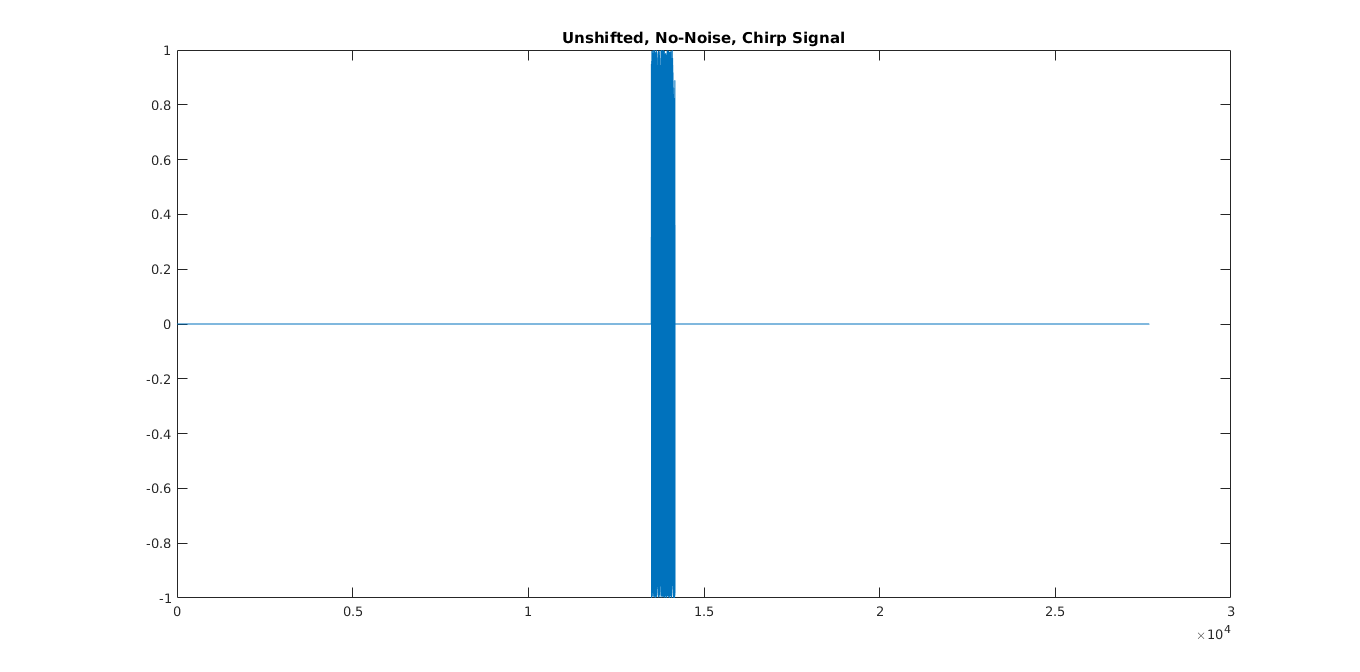
\includegraphics[width=1\linewidth]{./images/unshifted_no_noise_chirp.png}
      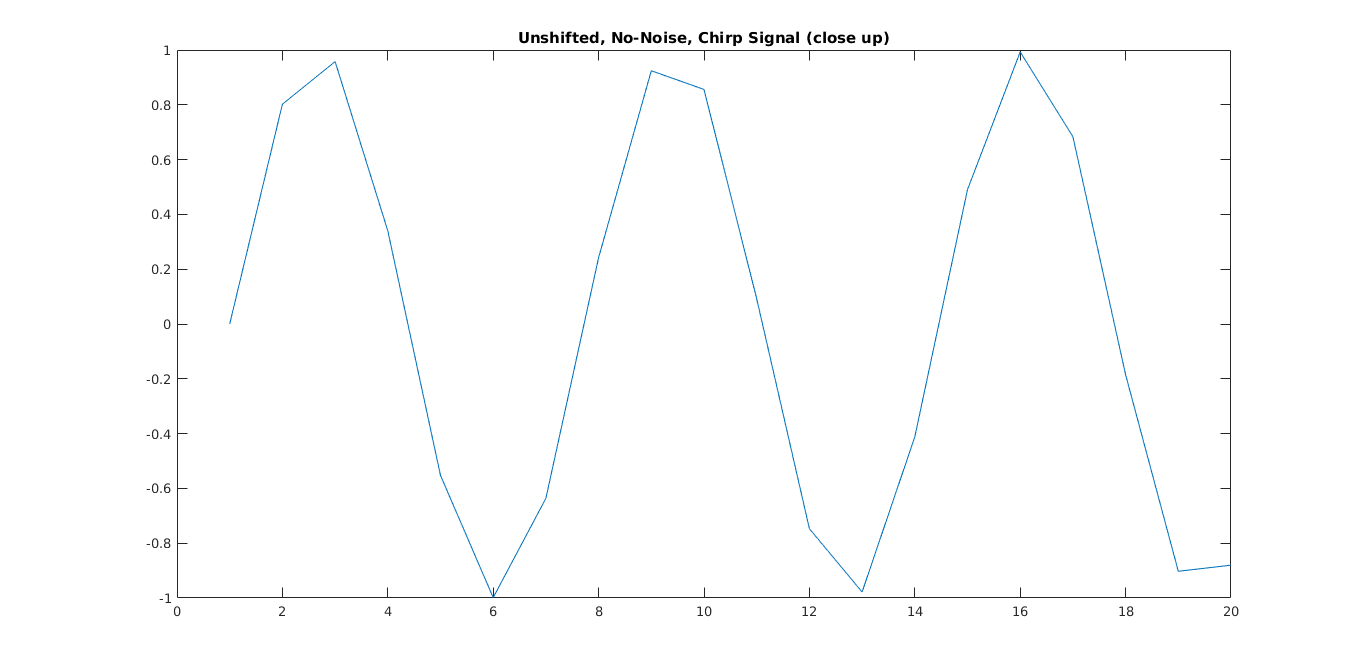
\includegraphics[width=1\linewidth]{./images/unshifted_no_noise_chirp_zoomed.png}
      \caption{Unshifted, No-Noise, Chirp, 20-27\SI{}{\kilo\hertz}}
      \label{fig:unshifted_no_noise_chirp}
    \end{figure}

    Given this original signal, we then pad the signal and add noise. The result of this is shown in figure \ref{fig:repeated_signal}. Finally, use our original clear signal as a pattern, and convolve it with our signal. The result of this is shown in figure \ref{fig:pattern_matching}.

    \begin{figure}
      \centering
      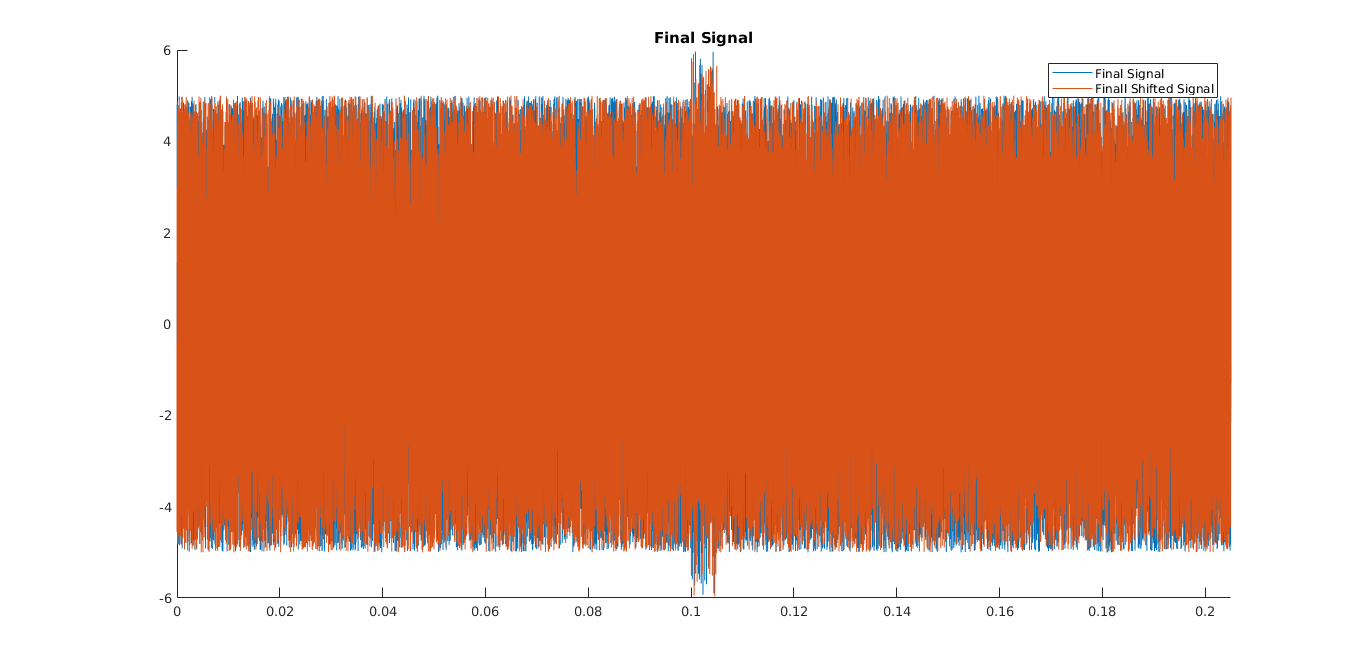
\includegraphics[width=1\linewidth]{./images/repeated_noisy_signal.png}
      \caption{Both the doppler-shifted and unshifted full noisy signals.}
      \label{fig:repeated_signal}
    \end{figure}

    \begin{figure}
      \centering
      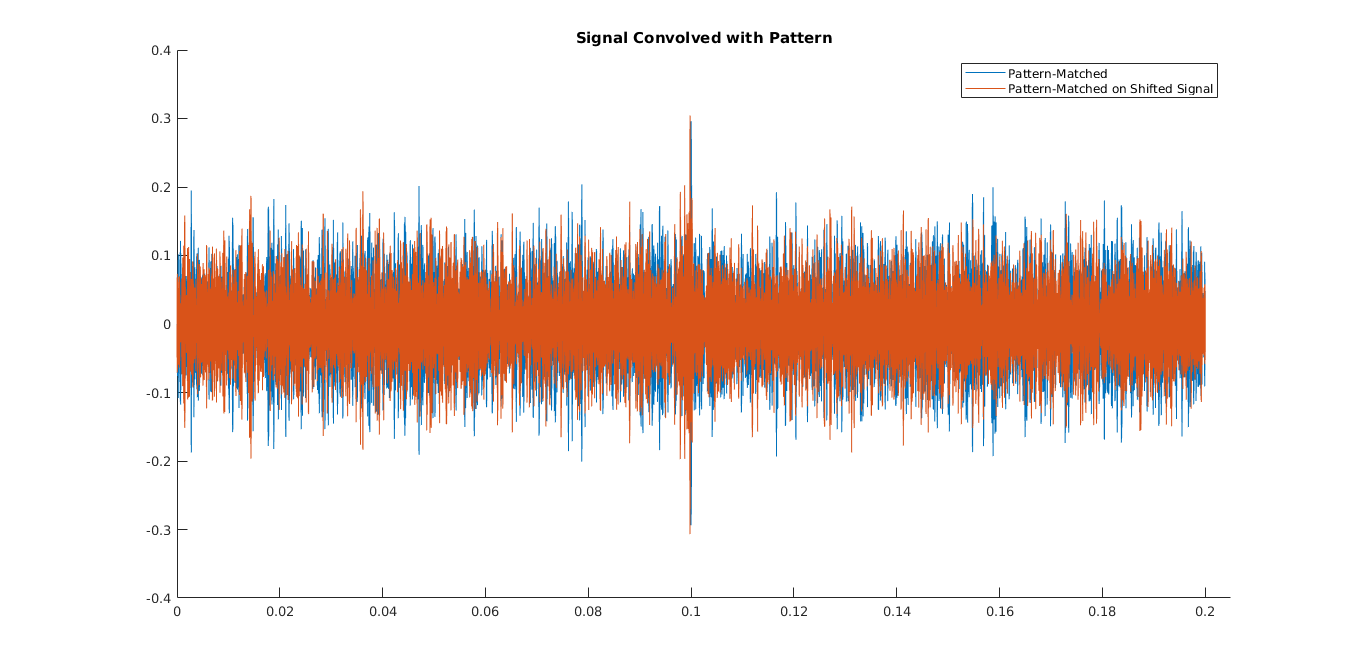
\includegraphics[width=1\linewidth]{./images/pattern_matching.png}
      \caption{The peaks in the center indicate the pattern matching the noisy signals closely.}
      \label{fig:pattern_matching}
    \end{figure}

    \subsubsection{The Doppler Effect on Ultrasonic}

      Using these simulated chirps, we ask the question of whether the doppler effect of a moving FRC robot will make the signal undetectable with simple pattern matching. The plots above show what happens if a doppler shift of a robot moving \SI{5}{\meter\per\second} is introduced. This speed causes a doppler shift of \SI{291.3}{\hertz}, and after applying pattern matching using the unshifted filter we see that the chirp is detected \SI{192.5}{\micro\second} early, which corresponds to \SI{6.6}{\centi\meter} of error, which is within our requirements (see section \ref{section:system_spec}). Furthermore, when the doppler has no effect, the error of our simulated detection is just \SI{2.5}{\milli\meter}, which is well within our requirements.

    \subsubsection{Effect of Chirp Bandwidth}

      One of the main limiting factors of using cheap piezo speakers is the limited range of frequencies that induce a measurable response (see \ref{section:frequency_response}. Using our simulated chirps, we experimented with changing the frequency range over which the chirps sweep. When we use the full range of 20-27\SI{}{\kilo\hertz}, the amplitude of the match filter is higher and the error is lower. However, when a smaller range such as 23-24\SI{}{\kilo\hertz} is used, the amplitude of the match filter is lower, and more difficult to distinguish with a simple threshold. For the implementation of a beacon system, this means that the chirps should span as wide a frequency range as possible.

  \subsection{Detecting Ultrasonic Signals on the PSoC 5LP}

    %FIXME: I'm not sure this section is relavent because we aren't usin the VDAC and we haven't tested its speed limits (1Msps according to datasheet)
    %\subsubsection{Limits of the ADC and DAC on the PSoC 5LP}

    %The VDAC8 on the psoc 5LP is limited by its speed setting options. There are only two options for what speed the DAC can be set to which are slow and high. The datasheet says that the slow option makes the settling time slower but consumes less operating current and the high mode does the opposite. The datasheet provides no further information about these settings so there is not a provided way to know the speed of the DAC. The DAC also is only 8 bit it can only be set to values between 0 and 255 which has not yet been a problem but is a limiting factor in general.
    %The Delta Sigma ADC has a resolution range of 8-20 bits.The lower the resolution the larger the range for conversion rate in samples per second. But even with the lowest resolution of 8 bits the range is only 8000-192000 which limits the minimum and maximum sample rate that can be used.

  \subsection{Ultrasonic Beam Angle \& Full Pattern}

    % could at do beam-spread equation here

  \subsection{Characteristics of Piezo Transducers}

    Throughout this project we also discovered several interesting characteristics of our piezo speakers. First, we note that emitting square versus sine waves does not seem to effect the received signal, given the same amplitude and frequency. We tested this by connecting on piezo to a function generator and another to an oscilloscope. We generated a high frequency wave, toggling between either square or sine wave, and compared the received waveform on the oscilloscope. By simply looking at the waveform, we were unable to determine whether the function generator was in square or sine wave mode. This means that even if the transmitting speaker is being moved like a square wave, the receiving transducer will simply resonate at the same frequency and the received signal will be a sinusoidal wave. This impacts implementation because square waves can be produced with high-precision digital components rather than analog components like DACs, so one may choose to use a square wave instead of a sine wave.

	\subsection{Co-Processors for Image Processing}

    Since our system requires processing of images from a video stream, we evaluated the Raspberry Pi 3 and the NVidia TK1 as potential co-processors. We ruled out the RoboRIO for image processing because many teams in FRC have found the RoboRIO insufficient for vision processing, and because we did not intend for computational efficiency to be a key criteria of this project. Further still, using a coprocessor allows us to write and run whatever our system requires, irrespective of how any teams actual robot code is operating.

    % FIXME: More testing here. How high FPS/resolution can we get on each platform?

  \subsection{Evaluting The Placement of ArUco Tags} \label{section:tag_placement}

    When doing localization with ArUco markers, generally the more markers that can be detected the better your pose estimates and maps will be. However, this is also a trade off with the amount of modification required in the environment. We would like to have as few tags as possible in our environment to minimize the amount of work required to localize in that environment. To begin to answer this question, we consider how the spacing between tags on a mock FRC field effects the detection rate of tags.

    \begin{figure}[H]
      \centering
      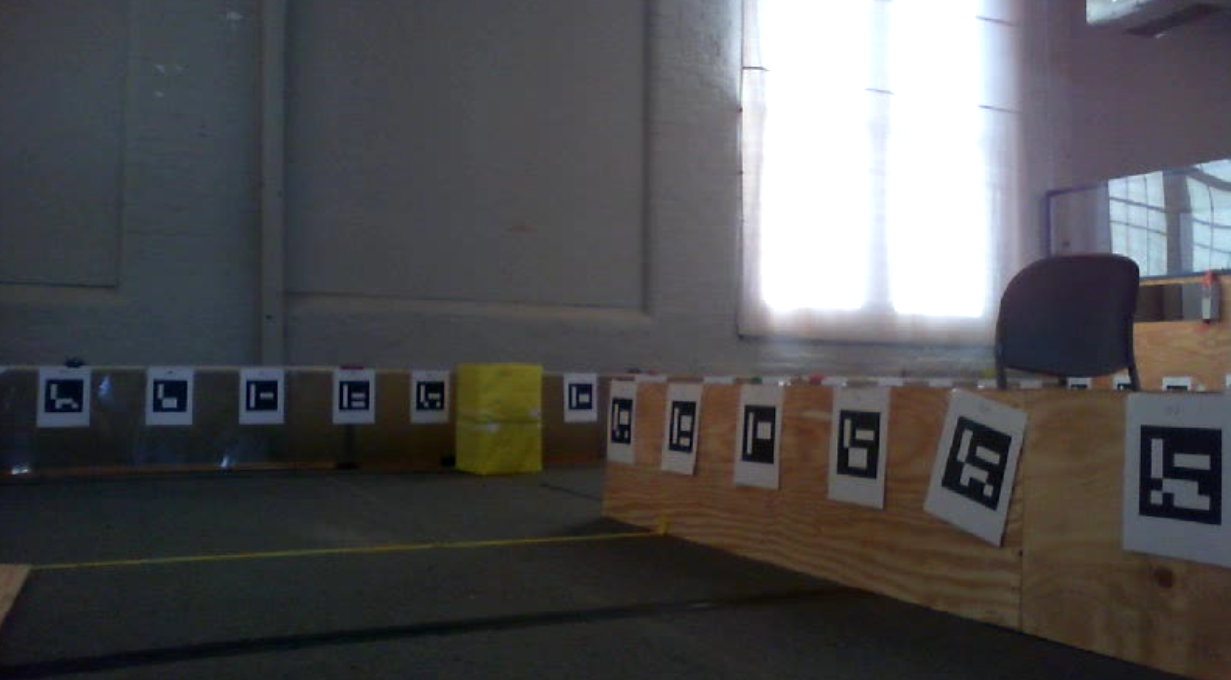
\includegraphics[width=1\linewidth]{./images/nypro_tag_spacing.png}
      \caption{Tags placed on the Nypro practice field}
      \label{fig:nypro_tag_spacing}
    \end{figure}

    We placed \SI{0.152}{\meter} tags every 1.5ft on a mock FRC field at Nypro (see Figure \ref{fig:nypro_tag_spacing}). We recorded video driving realistically around the field and counted how frequently we detected ArUco tags. We then filtered out tags by their ID numbers to simulate spacings of 3ft, 4.5ft, and 6ft. We report detection statistics for each of these spacings based on two different runs through the field in Table \ref{table:spacing_timing}. We also plot all the times between detections over the course of one of our runs in Figure \ref{fig:spacing_timing}. Our results show that, assuming reasonable camera settings of 480p30 (640x480, 30fps), the frequency of tag detection is essentially unchanged between 1.5ft and 6ft spacings. The only notable difference is the mean time between detections slowly rises as tags become further apart. Intuitively, this means that even 6ft between tags is close enough to expect to detect tags 10 times a second. More specifically, we can say that 95\% of the time we will detect a tag every \SI{0.1}{\second}. We do note that during our first trial, where our camera was accidentally only recording frames at 480p8, the tag detection rate suffers more significantly as tag detection increases.

    \begin{table}[H]
      \centering
      \begin{tabular}{|c|c|c|c|c|c|c|c|c|} \hline
        spacing (ft) & \multicolumn{2}{c}{worst case (s)} & \multicolumn{2}{c}{95th percentile (s)} & \multicolumn{2}{c}{mean (s)} & \multicolumn{2}{c|}{median (s)} \\ \hline
            & trial 1 & \textbf{trial 2} & trial 1 & \textbf{trial 2} & trial 1 & \textbf{trial 2} & trial 1 & \textbf{trial 2} \\ \hline
        1.5 & 5.100 & \textbf{3.700} & 0.762 & \textbf{0.068} & 0.235 & \textbf{0.053} & 0.132 & \textbf{0.032} \\ \hline
        3.0 & 5.231 & \textbf{3.700} & 0.932 & \textbf{0.100} & 0.269 & \textbf{0.061} & 0.132 & \textbf{0.032} \\ \hline
        4.5 & 5.900 & \textbf{3.700} & 1.145 & \textbf{0.100} & 0.284 & \textbf{0.064} & 0.132 & \textbf{0.032} \\ \hline
        6.0 & 7.832 & \textbf{3.700} & 1.343 & \textbf{0.100} & 0.335 & \textbf{0.070} & 0.132 & \textbf{0.032} \\ \hline
      \end{tabular}
      \caption{Tag detection metrics compared across tag spacings.
      The larger spacings have slightly worse performance, but still usually provide updates at least 10 timers per second.
      Trial 1 only recorded at 8fps, but is included for completeness. Trial 2 was 30fps.}
      \label{table:spacing_timing}
    \end{table}

    \begin{figure}[H]
      \centering
      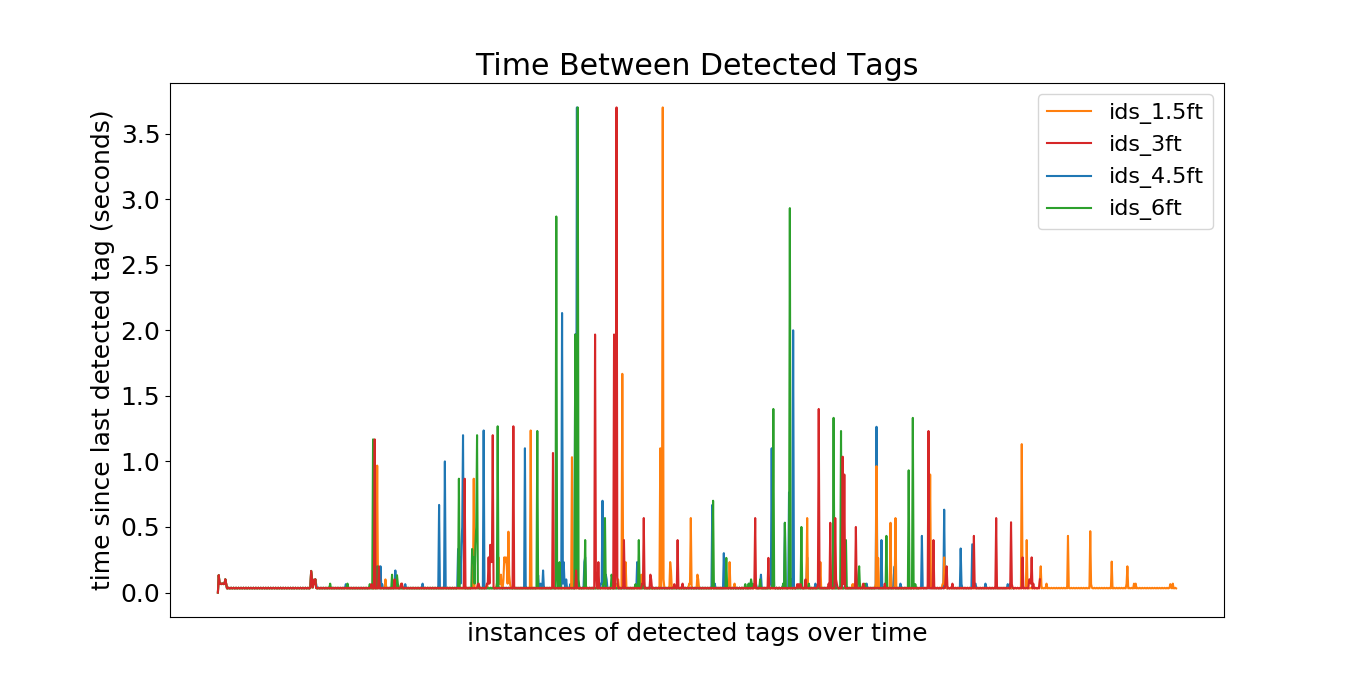
\includegraphics[width=1\linewidth]{./images/spacing_times.png}
      \caption{Times between detected tags as a function of tag spacing. Spacings between 1.5ft and 6ft perform very similarly.}
      \label{fig:spacing_timing}
    \end{figure}


    It is important to note several other factors that are not explored here, including how spacing and positioning effects the accuracy of detections. Furthermore, one should ask whether the specific locations of tags, not just the spacing between them, also effects detection accuracy and frequency. Intuitively, we claim that tags should be placed in locations where the robots camera is likely to be facing, such as feeding stations and goals. However, we do not empirically evaluate this claim.

	\subsection{Statistics of CSCore Image Timestamps}

    We use the built-in API of CSCore to get the time stamps (in microseconds) for each image captured. During many of our tests, we logged these times to files for offline processing. We now ask how much these time stamps vary from the requested FPS. This is important information to know, because it effects whether or not one can assume a truly constant FPS. We find that there is significant variation between any individual frames. Table \ref{table:fps_stats} shows key statistics about FPS over a multitude of recordings from our test robot. These recordings are taken from our tests at Nypro, with various requested frame rates and at various resolutions.

    \begin{table}[H]
      \centering
      \begin{tabular}{|c|c|c|c|c|c|} \hline
        Requested FPS & Resolution & Mean FPS & Median FPS & Min FPS & Max FPS \\ \hline
        30 & 1920x1080 & 14.90 & 14.71 & 9.61 & 22.75 \\ \hline
        30 & 1920x1080 & 15.11 & 14.71 & 10.00 & 27.83 \\ \hline
        30 & 1280x720 & 8.17 & 7.59 & 2.29 & 14.78 \\ \hline
        30 & 1280x720 & 8.35 & 7.60 & 2.00 & 14.75 \\ \hline
        30 & 800x448 & 29.34 & 31.08  & 4.31 & 31.78 \\ \hline
        60 & 640x480 & 59.43 & 60.02 & 3.53 & 62.48 \\ \hline
        60 & 640x480 & 59.71 & 60.02 & 3.33 & 89.32 \\ \hline
        30 & 640x480 & 30.00 & 30.01 & 3.76 & 30.13 \\ \hline
        30 & 320x240 & 30.04 & 31.21 & 2.72 & 31.71 \\ \hline
        30 & 320x240 & 30.03 & 31.22 & 3.33 & 32.30 \\ \hline
        30 & 320x240 & 30.08 & 31.21 & 14.76 & 32.69 \\ \hline
      \end{tabular}
      \caption{Table of statics from a multitude of CSCore streams. We find that FPS can vary throughout normal operation.}
      \label{table:fps_stats}
    \end{table}

    We observe that startup-lag is the true cause of low minimum FPS, and therefore does not cause significant issues unless pose estimates from the first two frames are critical. However, there are in fact cases where the camera exceeds the desired FPS but as much as 48\% in the case of 60fps. There are also several cases where the processing collecting and stamping these images was not powerful enough to acheive the requested FPS. For example, we requested 720p30 on a raspberry pi, but were only able to capture at $\approx$15fps. This is real constraint that must be handled in a camera based localization system, and so we report those results for completeness. However, our results show that, assuming the computer is powerful enough to acheive the requested FPS on average, there are only small variations on FPS over time. We provide two full plots of FPS over time in two of the more curious entries in table \ref{table:fps_stats} to be more illistrative of how time between frames can vary (figures \ref{fig:fps_plot_1} and \ref{fig:fps_plot_2}).

    \begin{figure}[H]
      \centering
      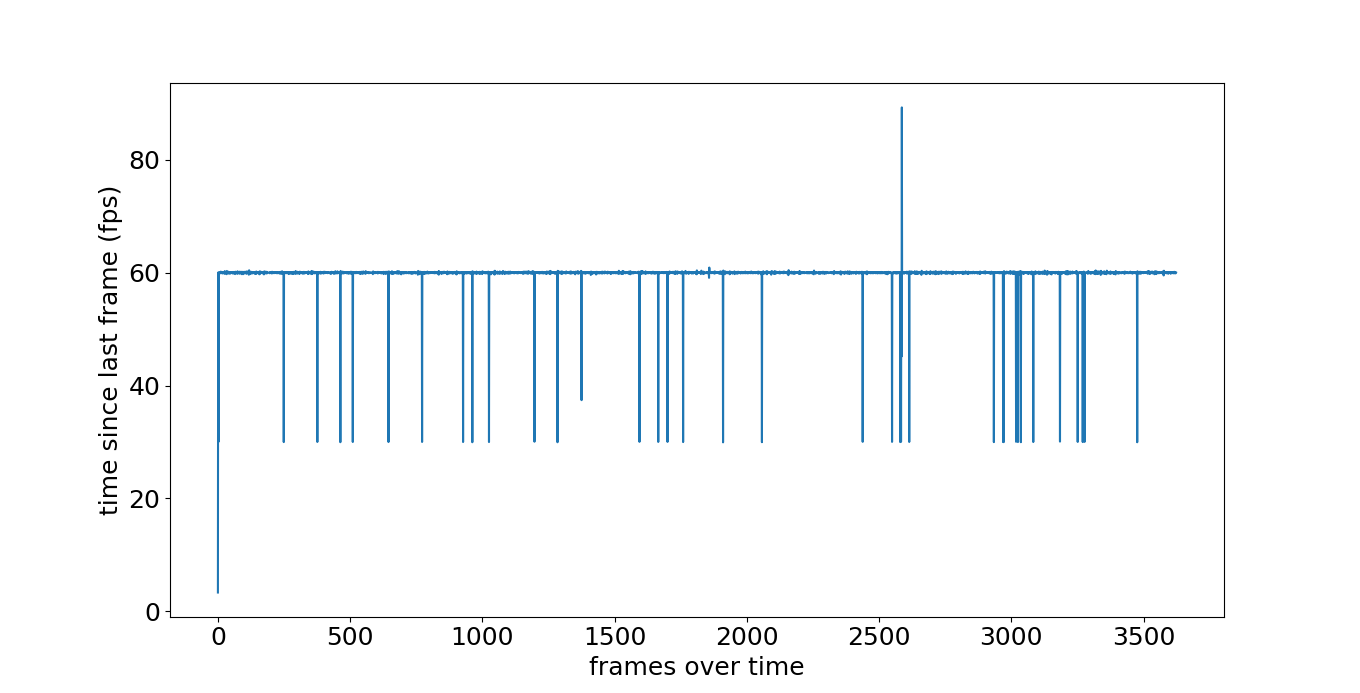
\includegraphics[width=0.8\linewidth]{./images/fps_plot_2.png}
      \caption{FPS over time for one instance of 240p30}
      \label{fig:fps_plot_2}
    \end{figure}

    \begin{figure}[H]
      \centering
      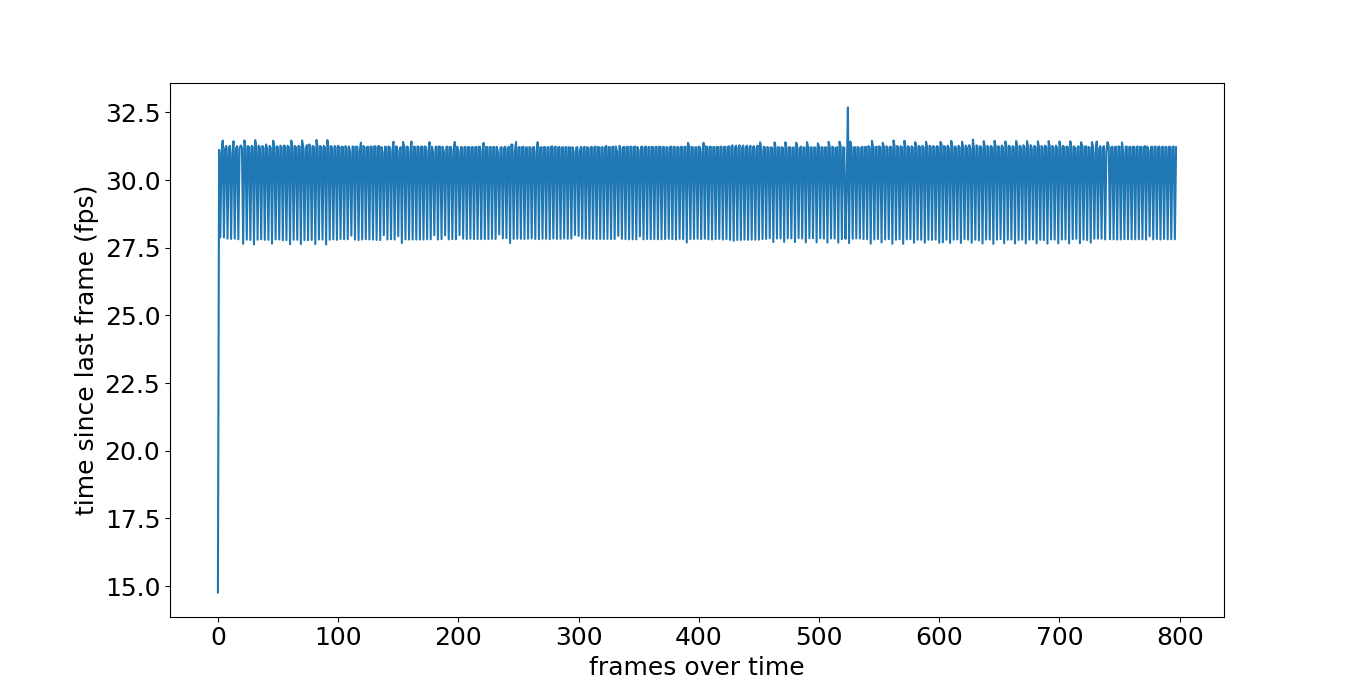
\includegraphics[width=0.8\linewidth]{./images/fps_plot_1.png}
      \caption{FPS over time for one instance of  480p60}
      \label{fig:fps_plot_1}
    \end{figure}

	\subsection{Effect of Frame Rate and Resolution on ArUco Tag Detection}

    We explore the effect of frame rate and resolution on the frequency with which tags are detected. This frequency of detected tags is an important metric because it sets the standard for how long our dead-reckoning methods must run without receiving an update to compensate for drift. Furthermore, since the FPS and resolution of a camera correlates with cost, we want to know whether a cheap camera is sufficient for tag detection.

    To answer this question, we used three cameras simultaneously recording footage from the robot as we drove around a mock FRC Field. It is important that these cameras are recording simultaneously and are mounted right next to each other, because it means the camera streams will see essentially the same view of the world, with the only variable being the resolution and FPS. The tags were placed roughly every 6 feet (according to results of section \ref{section:tag_placement}) and the robot was driven through a simulated FRC game for \SI{60}{\second}. We then compare how frequently tags were detected by looking at gaps between detections. Table \ref{table:tag_detection_comparison} shows a comparison of various key metrics between the different resolution/FPS pairings. The full plots showing all gaps in the run is shown in appendix \ref{appendix:tag_detection}

    \begin{table}[H]
      \centering
      \begin{tabular}{|c|c|c|c|c|c|} \hline
        Condition & Worst-Case & 95th percentile & Mean & Median & Mode \\ \hline
        PS4 Eye 480p30 & 4.565 & 0.100 & 0.062 & 0.033 & 0.033 \\ \hline
        PS4 Eye 480p60 & \textbf{3.049} & \textbf{0.033} & \textbf{0.032} & \textbf{0.017} & \textbf{0.017} \\ \hline
        C920 1080p15 & 3.196 & 0.767 & 0.162 & 0.068 & 0.068 \\ \hline
      \end{tabular}
      \caption{480p30 means 640x480 at 30fps, 480p60 means 640x480 at 60fps, 1080p15 means 1920x1080 at 15fps. The best settings by all measures was the PS3Eye camera at 60fps.}
      \label{table:tag_detection_comparison}
    \end{table}

    Arguably the most important metric here is the 9th percentile metric, which says that 95\% of of the time gaps between detected tags are less than that number. Generally, that number is quite close to the mean frame rate which means that usually you get one tag detected in every frame, but this is of course not always true. It's important to note that just because a there was a tag detected in the frame doesn't mean we get a reliable position estimate from that tag. So these numbers are not the same as the how frequently an actual position is received, which is what we truly care about.

    In conclusion, the 480p60 setting performs the best by all metrics, and therefore we recommend using those settings.

  \subsection{Rate of position estimates from ArUco Tags}

    Although the detection of tags, is important, what is really important is the estimates of their pose. We now consider only valid position estimates, and not just any detected tag, and measure the frequency of pose estimates from our camera. We use the same recordings at the Nypro test field as we have used throughout this report, and similar to section \ref{section:tag_placement} we compare the time between valid pose estimates. For completeness, we also compare this across the three resolution/fps settings which were recorded. One notable oddity in the data is the extremely high variance in the worst-case time between pose detections across trials and tag spacings. We simulated tag-spacings by filtering out tags based on their IDs, which is accurate because tags were placed in order. However, it means that it's possible for a tag that is present in more sparsely spaced group (ex: 6ft) to be missing from densely spaced group (4.5ft). We can explain this high variance by saying that there was a tag included in the 6ft spacing test that was not present in the 4.5ft spacing test, and without that tag there is a longer period in which no tags are seen. Secondly, we can also say that the high variance between the two trials is explained by the different paths the robot took in each trial. This is a very important result, because it means that depending on how a robot moves through the field, the frequency of valid pose estimates will change.

    \begin{table}[H]
      \centering
      \begin{tabular}{|c|c|c|c|c|c|c|c|c|} \hline
        spacing (ft) & \multicolumn{2}{c}{worst case (s)} & \multicolumn{2}{c}{95th percentile (s)} & \multicolumn{2}{c}{mean (s)} & \multicolumn{2}{c|}{median (s)} \\ \hline
            & trial 1 & trial 2 & trial 1 & trial 2 & trial 1 & trial 2 & trial 1 & trial 2 \\ \hline
            1.5ft & 2.7960 & 3.1961 & 0.2420 & 0.7736 & 0.1135 & 0.1623 & 0.0680 & 0.0680 \\ \hline
            3ft   & 3.5960 & 4.0040 & 0.9228 & 0.9680 & 0.1804 & 0.1958 & 0.0680 & 0.0680 \\ \hline
            4.5ft & 6.5961 & 6.4640 & 1.0160 & 1.2224 & 0.2316 & 0.2556 & 0.0680 & 0.0680 \\ \hline
            6ft   & 10.7960 & 4.7259 & 0.8038 & 1.1300 & 0.2703 & 0.2625 & 0.0680 & 0.0680 \\ \hline
      \end{tabular}
      \caption{Statistics of Pose Estimates from two trials of 1080p15 footage, across various tag spacings. Note the high variance in worst-case across.}
      \label{table:480p30_pose_estimate_stats}
    \end{table}

    \begin{table}[H]
      \centering
      \begin{tabular}{|c|c|c|c|c|c|c|c|c|} \hline
        spacing (ft) & \multicolumn{2}{c}{worst case (s)} & \multicolumn{2}{c}{95th percentile (s)} & \multicolumn{2}{c}{mean (s)} & \multicolumn{2}{c|}{median (s)} \\ \hline
            & trial 1 & trial 2 & trial 1 & trial 2 & trial 1 & trial 2 & trial 1 & trial 2 \\ \hline
        1.5ft & 1.5161 & 3.0489 & 0.0334 & 0.0334 & 0.0295 & 0.0324 & 0.0167 & 0.0167 \\ \hline
        3ft   & 1.5161 & 5.8312 & 0.0500 & 0.0334 & 0.0437 & 0.0448 & 0.0167 & 0.0167 \\ \hline
        4.5ft & 2.9823 & 7.2807 & 0.0333 & 0.0333 & 0.0479 & 0.0553 & 0.0167 & 0.0167 \\ \hline
        6ft   & 2.2492 & 6.9642 & 0.0334 & 0.0334 & 0.0445 & 0.0533 & 0.0167 & 0.0167 \\ \hline
      \end{tabular}
      \caption{Statistics of Pose Estimates from two trials of 480p60 footage, across various tag spacings.}
      \label{table:480p30_pose_estimate_stats}
    \end{table}

    \begin{table}[H]
      \centering
      \begin{tabular}{|c|c|c|c|c|c|c|c|c|} \hline
        spacing (ft) & \multicolumn{2}{c}{worst case (s)} & \multicolumn{2}{c}{95th percentile (s)} & \multicolumn{2}{c}{mean (s)} & \multicolumn{2}{c|}{median (s)} \\ \hline
            & trial 1 & trial 2 & trial 1 & trial 2 & trial 1 & trial 2 & trial 1 & trial 2 \\ \hline
        1.5ft & 3.6987 & 4.5651 & 0.0666 & 0.1000 & 0.0517 & 0.0621 & 0.0333 & 0.0333 \\ \hline
        3ft   & 4.8316 & 5.8313 & 0.0667 & 0.1999 & 0.0711 & 0.0899 & 0.0333 & 0.0333 \\ \hline
        4.5ft & 8.1971 & 7.1642 & 0.0766 & 0.1500 & 0.1206 & 0.1104 & 0.0333 & 0.0333 \\ \hline
        6ft   & 10.4296 & 6.8976 & 0.1483 & 0.1517 & 0.1164 & 0.0959 & 0.0333 & 0.0333 \\ \hline
      \end{tabular}
      \caption{Statistics of Pose Estimates from two trials of 480p30 footage, across various tag spacings.}
      \label{table:480p30_pose_estimate_stats}
    \end{table}

    If we consider the 59th percentile metric as our most important metric, we should ask what spacing and resolution/fps settings give acceptably fast update rates. If we desire updates at least every \SI{0.1}{\second} (see section \ref{section:design_criteria} for justification), then we say that 480p60 will be sufficient at any of the tested tag spacings. On the other hand, 1080p15 gives update too infrequently no matter how close tags are spaced. This makes sense, because at 15fps, a tag would need a valid pose estimate in essentially every frame to acheive \SI{0.1}{\second} update rate. Lastly, we can say that 480p30 probably would work with 1.5ft and 3ft spacings, and it becomes slightly too slow at 4.5ft and 6ft spacings. Ultimately, we recommend using 480p60, and suggest a 6ft spacing so as to minimize the modification of the environment.

    % also compare position estimates between each of the cameras
    % compare graphically over time
    % compare individual points in frames
    % compare covariance after Kalman filtering

	\subsection{Benchmarking MarkerMapper with VICON Motion Capture}

	\subsection{On Building MarkerMaps}

	\subsection{Erroneous detections with ArUco}

    Marker Maps must comprise fiducial markers from known "dictionaries" or binary encodings. Examples of a several dictionaries are shown below. Dictionary selection is important because it allows users to optimize their Marker Maps. Users can choose dictionaries with different numbers of tags, marker (square) sizes, and inter-marker distances. Inter-marker distances are determined by the number of tags in the dictionary (high distances correspond to low numbers of tags). High inter-marker distances make detection more robust. Tags are defined by a list of bytes which determine the color of squares. Dictionaries can be further optimized by setting the "maxCorrectionBits" parameter experimentally to reduce false positives\cite{open_source_computer_vision_detection_2015}.

    Throughout our experiments with ArUco tags, we accumulated several examples of detections that were erroneous in some form or another. First, we present examples of tags whose ID is misdetected (Figure \ref{fig:misdetected_tags}). In all these cases the incorrectly detected ID was 2, but there is no evidence that this is an issue just with tag 2 specifically.

    \begin{figure}[H]
      \centering
      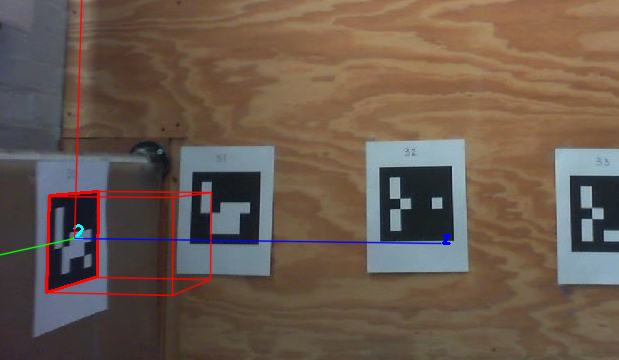
\includegraphics[width=0.49\linewidth]{./images/misidentified_tag_1.png}
      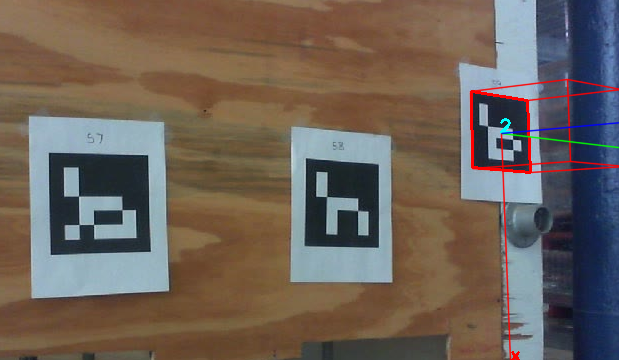
\includegraphics[width=0.49\linewidth]{./images/misidentified_tag_2.png}
      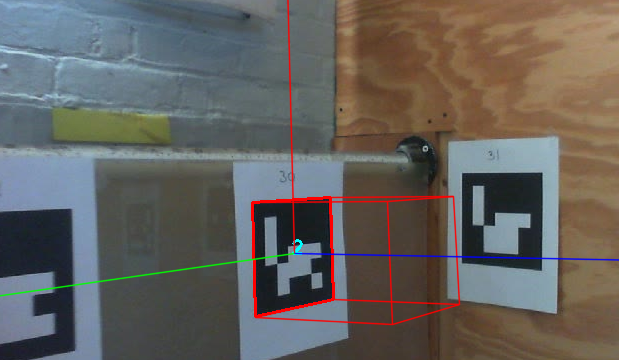
\includegraphics[width=0.49\linewidth]{./images/misidentified_tag_3.png}
      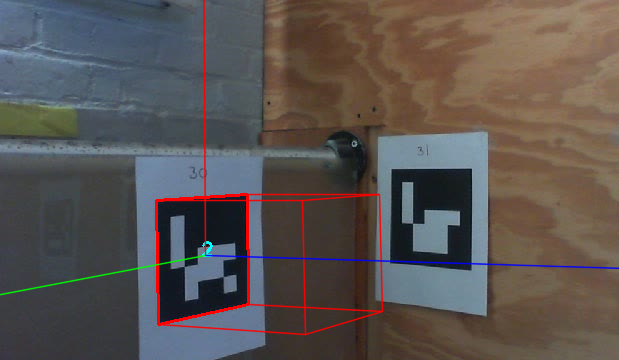
\includegraphics[width=0.49\linewidth]{./images/misidentified_tag_4.png}
      \caption{Tags that were detected, but with the wrong IDs}
      \label{fig:misdetected_tags}
    \end{figure}

    We also report how a poor camera calibration file and cause inaccuracies in the estimated poses of tags. In Figure \ref{fig:bad_tag_pose}, the tag's ID is identified correctly, but it's orientation is incorrect.

    \begin{figure}[H]
      \centering
      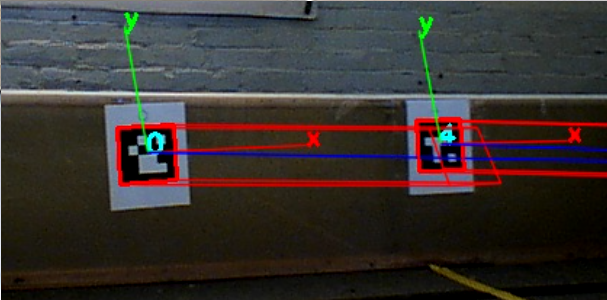
\includegraphics[width=1\linewidth]{./images/bad_tag_pose_1.png}
      \caption{Example of poor camera calibration file causing skewed pose estimate.}
      \label{fig:bad_tag_pose}
    \end{figure}

	\subsection{Latency over the Robot Network}

		It is important that all of our sensor data be time stamped so we can account for latency in our state estimation. The data collected on the NavX is time stamped on the NavX, and the encoder data is stamped when it is read on the RoboRIO. This time stamped data is sent to the TK1 over UDP. UDP was chosen because it was the easiest method with satisfactory speed. To test this, we wrote a simple program that sends 96 bytes, an upper bound on the size of all our stamped sensor data, of UDP data between the RoboRIO and the TK1. We recorded the round trip time of these packets, which can be seen in Figure \ref{fig:udp_timing}. The round-trip latency was \SI{0.5}{\milli\second} on average, which is much faster than any of our sensors, and therefore is fast enough for us to transmit and process the data before new data arrives.

		\begin{figure}[H]
			\centering
			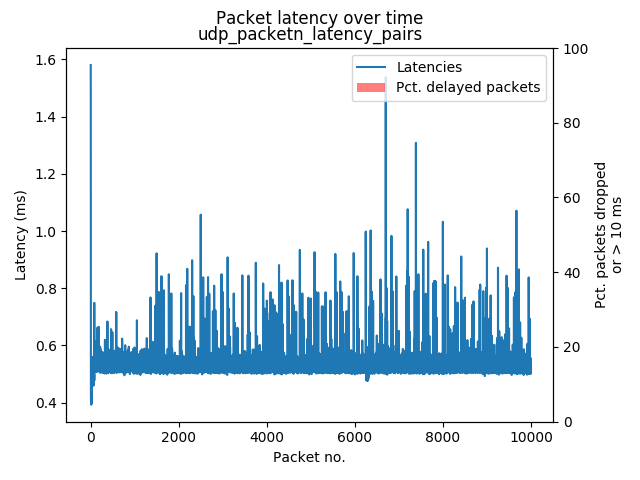
\includegraphics[width=0.7\linewidth]{./images/rio_tk1_udp_latency_timeseries.png}
			\caption{RTT of UDP packets between the RoboRIO and the TK1 over the robot's wired network.}
			\label{fig:udp_timing}
		\end{figure}

		Another important problem is time synchronization. The time stamps on all the data must be in reference to some common time source. To achieve this effect, we use Christian's Algorithm \cite{cristian_probabilistic_1989}. Specifically, we send a packet stamped with the current time on the RoboRIO to the TK1, the TK1 adds its own time stamp and responses, the and RoboRIO then add half the round trip time to the time sent by the TK1. This allows the sensor data sent from the RoboRIO to be synchronized with the clock on the TK1.


\section{A Dataset for Robot Localization} \label{section:dataset}


\section{Sample Implementation} \label{section:specs}

  In order to evaluate the theory and research presented above, we built a complete localization system using an FRC Chassis (courtesy of our sponsor AndyMark), and NavX-MXP IMU (courtesy of Kauai Labs), encoders, and a PS3Eye webcam. In this section, we describe the details of this system and explain the lessons learned from implementing and testing the platform.

	\subsection{Robot Hardware}

    A picture of the robot we built can be seen in Figure \ref{fig:mocap_robot}. This robot consists of an AndyMark chassis (am-2240) with Toughbox gearboxes (similar to am-0977), and two sets of 6in wheels. The back wheels are have more traction than the front, which has the platform have more interesting and challenging dynamics--a simple Dubin's car or differential drive model is inaccurate. We use two Greyhill 63R256 encoders with 256 pulses per revolution. Because the gear ratio of our gearboxes is unknown, it was simpler to directly measure distance per pulse, which we found to be \SI{0.000375}{\meter} per pulse.


	\subsection{Kalman Filtering}

  \subsection{System Requirements}\label{section:system_spec}

    Based on the extensive literature review, the few preliminary experiments we've conducted, and our design criteria, we eliminated our initial list of possible techniques down to the following five:

    \begin{enumerate}
        \item Radio and ultrasonic beacons
        \item IMU
        \item Drive wheel encoders
        \item Optical flow
        \item Camera with matrix tags
    \end{enumerate}

    We have found examples of each of these techniques being used successfully, and in many cases have verified that they satisfy our criteria for accuracy, precision, update rate, and accessibility criteria. We are confident that any combination of these methods would work. These techniques are complementary in their sources of error, and together we believe they will make a robust localization system.

  \subsection{Implementation Details}

    Having decided on the sensing techniques we will use, we now describe our detailed system Specification. Ideally, the description in this section serves as the full plan for our implementation of the system during B Term, and most of the major design decisions have been made and clearly presented.

		\subsubsection{The Test Robot}

			This section describes the hardware and software of the test robots we used throughout our experiments. We use an old FRC Kit-of-parts Chassis with 6" wheels. The rear wheels have high-grip rubber and the front wheels are a slick hard plastic. This creates an interesting uneven turning center, which is a good test-platform for robots that slip when turning. We use two CIM motors to drive the wheels and two Talon speed controllers to drive the CIMs. Our robot also has a RoboRIO and an NVidia brand Jetson TK1, which are networked together with a COTS router. For sensing, we have two Greyhill 63R256 encoders, a cheap 720p USB webcam, and a NavX-MXP. Figure \ref{fig:mocap_robot} shows the fully assembled robot.

			\begin{figure}[H]
				\centering
				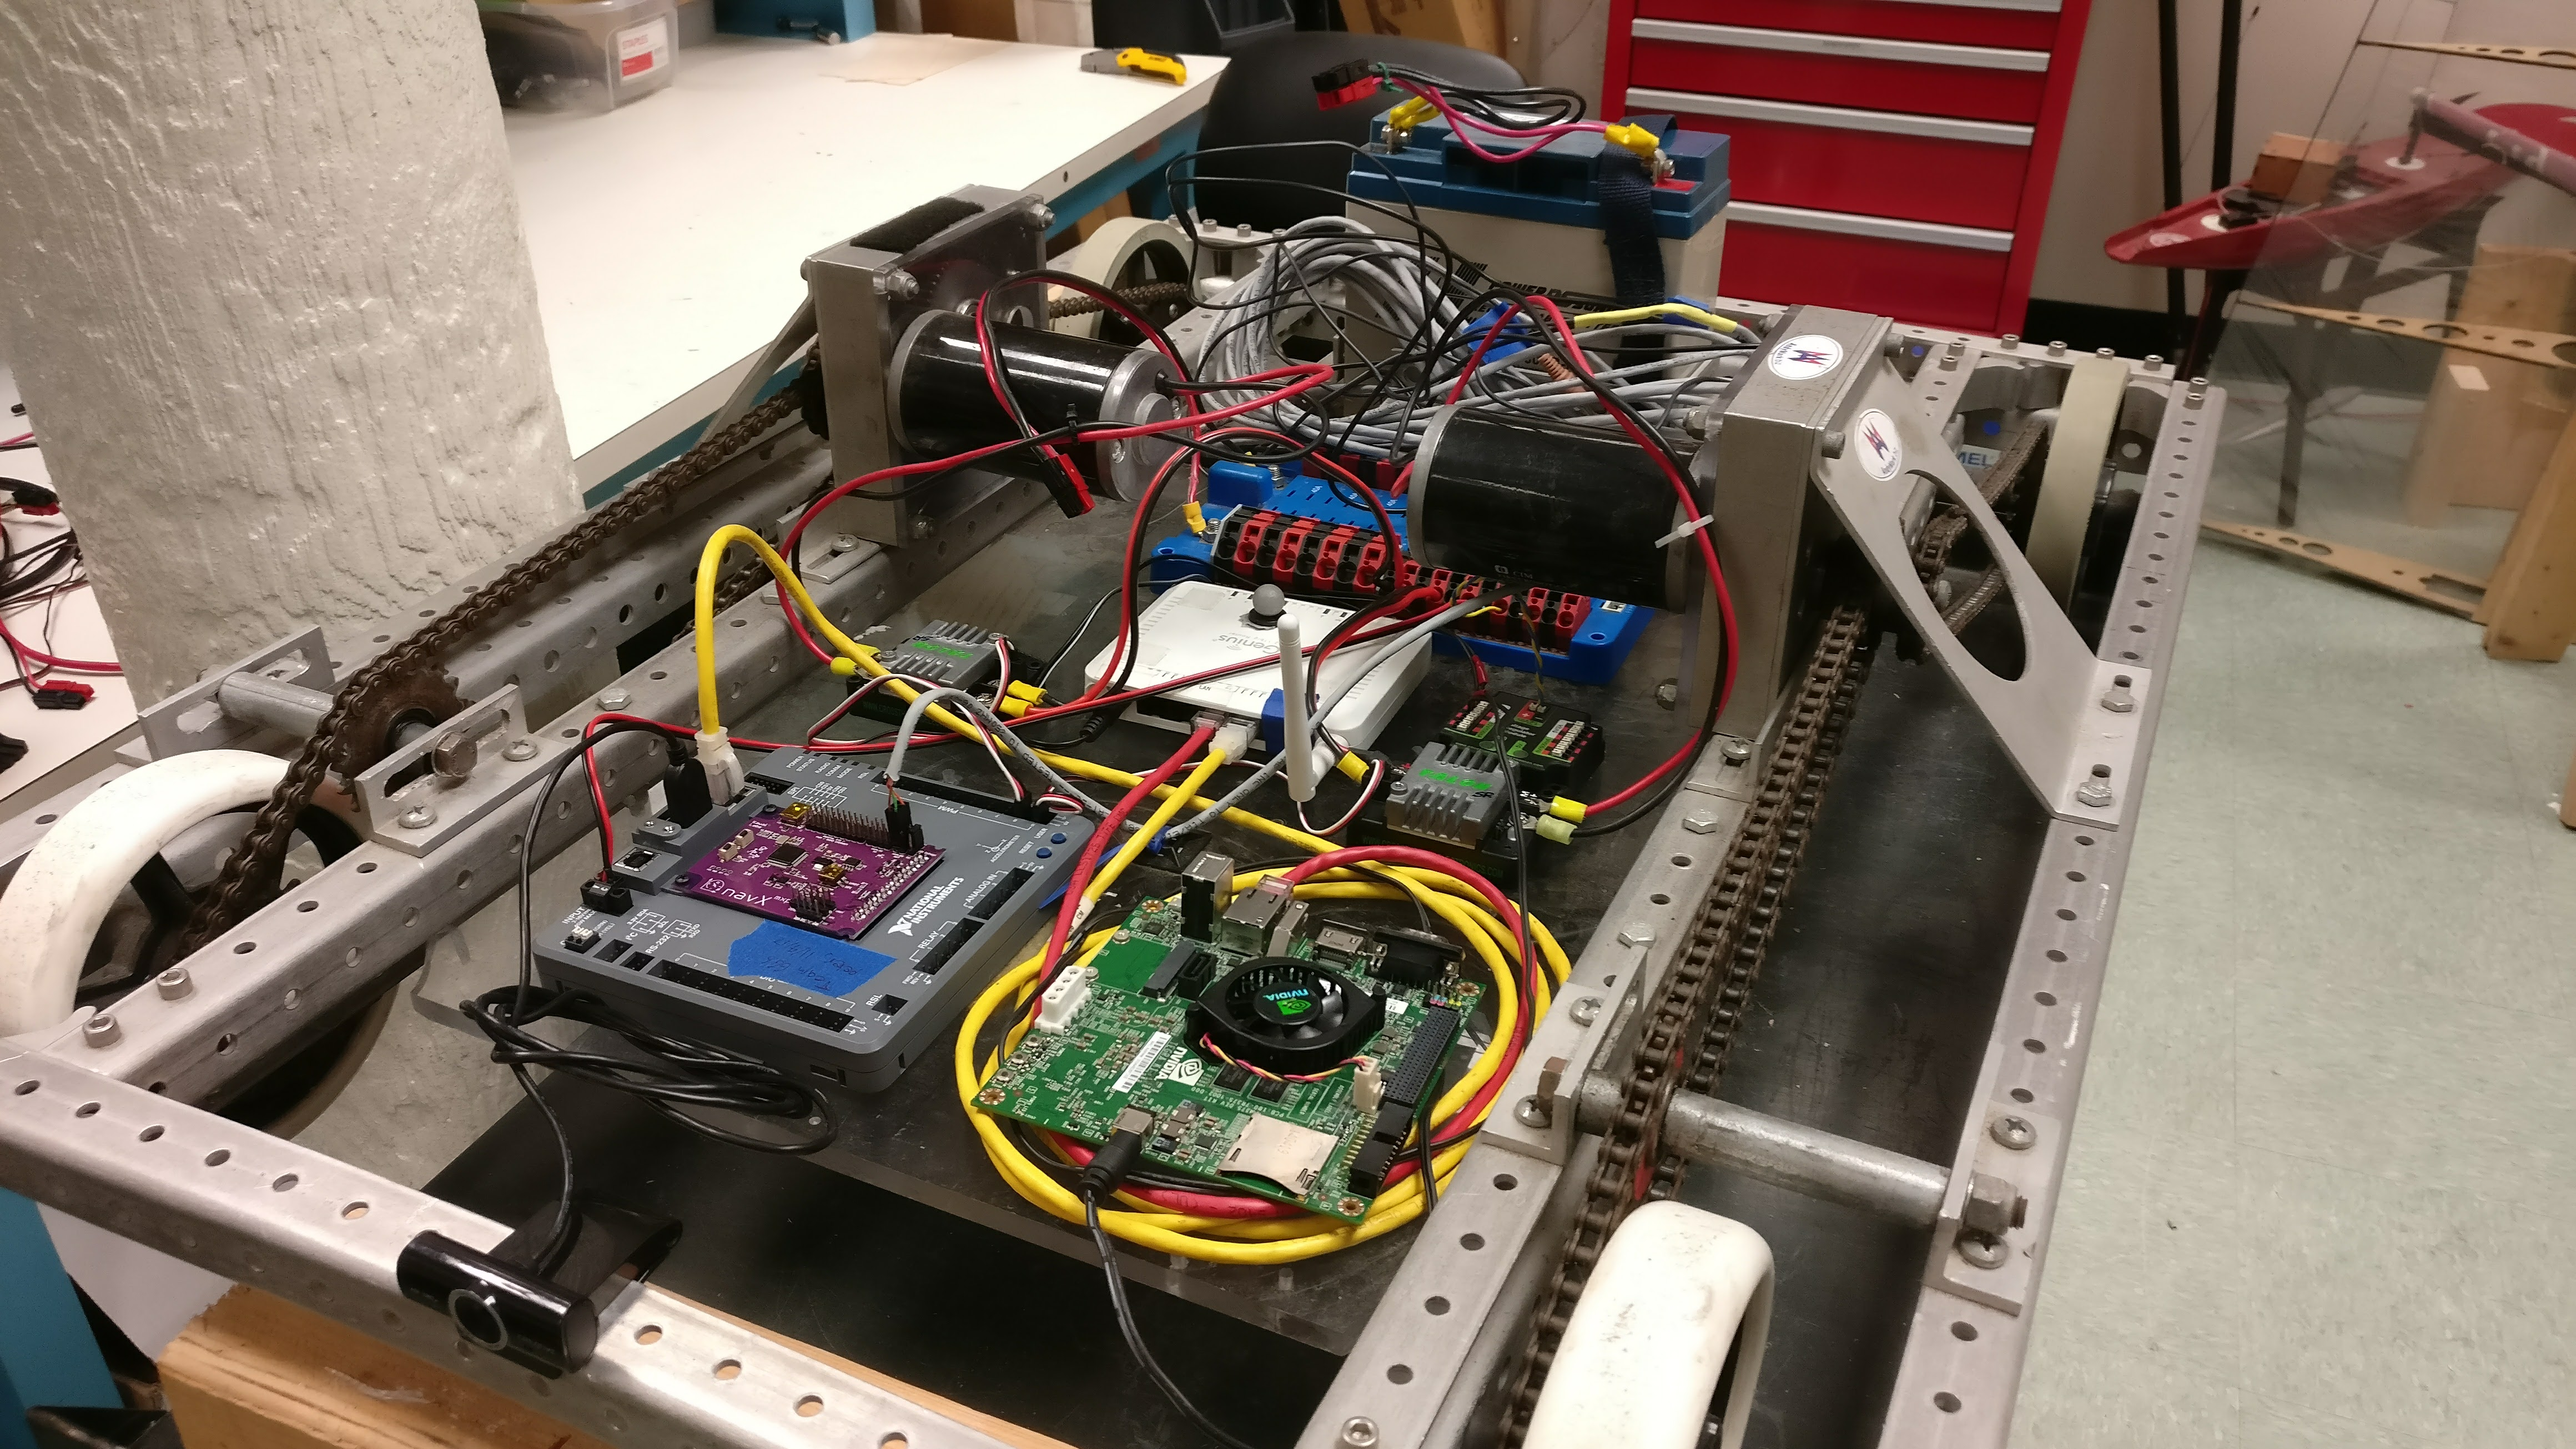
\includegraphics[width=1\linewidth]{./images/mocap_robot.jpg}
				\caption{Test Robot used in our experiments}
				\label{fig:mocap_robot}
			\end{figure}

			\subsubsection{General Architecture}

			Given the five sensing technologies mentioned above, we will now provide details on the configuration and use of each sensor. The Navx IMU is connected to the RoboRIO, which is the main processor which are FRC teams are required to use. The encoders on the drive train are similarly connected to the digital IO pins on the RoboRIO. These sensors are connected to the RIO directly because they are often used by FRC Teams in their robot programs. We also introduce the NVIDIA Jetson TK1 as a co-processor. The camera is connected via USB-A to the TK1. Because of its superior computational power, the TK1 is responsible for processing all of the raw sensor data and delivering the result back to the main robot program. In this setup, the TK1 can receive sensor data from the RoboRIO over the robot network band from the USB webcam directly.

			There are two software components of our system. First, there is a a C++ library cross-compile for the RoboRIO that FRC teams will use in their robot projects. Teams are expected to call two or three simple functions in their robot program, which gives us everything we need to log sensor data and send it to the TK1. Because of this minimal API, we require very few changes to robot programs in order to get localization. This will make it approachable for teams and encourage them to try localization. The second software component is a C++ program running on the TK1. This program reads the camera data, serves http camera streams, receives the sensor data from the RoboRIO, computes the position of the robot, and reports this position over network tables. Again, the TK1 was chosen for this task because of it's computing power.

    \subsubsection{Accelerometer Processing}

      % describe our final methods for what we're actually doing with the navx data

    \subsubsection{Encoder IMU Fusion}

      The fusion of Encoder and IMU data will be the foundation of our localization system. While we do not plan to explore it too deeply, it will be the first component we work on in B term. The sensors supported will be the Kauai Labs NavX MXP and Micro. The system will not prevent the user from interfacing with either sensor in other ways. The IMU and encoder toolkit will feature an interface for user to input information about their kinematic base, namely wheel radius, wheelbase length, and encoder resolution. Using this information, the system will generate a state space model comprising minimally position and velocity terms. The drivetrain configuration that will be supported is a differential four wheel drive. Support may later be offered for one omnidirectional configuration, such as H-Drive. Using this information, a Kalman and complementary filtering program will be developed. Inputing a sensor configuration in software will allow a team to display local trajectories using a 2-D visualization. The team must be able to quickly modify parameters such as the filtering function used or the radius of a wheel and recalibrate each sensor on-line. This portion of the project must be completed approximately at the start of the FIRST build season.



      \textbf{Calibration}

      \textbf{Description of the Robot Model}

    \subsubsection{Radio and Ultrasonic Beacons}

      Important implementation details of the beacon system include the number of beacons needed, the radio communications protocol, and the ultrasonic signal format. The number of beacons can either be picked to minimize cost, and then the beacons can be designed to meet this criteria, or the characteristics of the beacons can be determined and the number of beacons needed derived from that. In order to support arbitrary practice areas, the second method is preferred. In this section we cover relevant calculations and possible implementation details for beacons.

      \textbf{Overview of components}

      Each beacon consists of a PSoc5 LP processor, NTX-1004PZ piezo transducer, XY-MK \SI{433}{\mega\hertz} radio transmitter, XY-FST \SI{433}{\mega\hertz} radio receiver, and other supporting components. During normal operation, each beacon will listen for a radio signal telling it to emit an ultrasonic signal. We expect that a few other components such as resistors, LEDs, and a battery will be required for the final beacon.

      \textbf{Format for Ultrasonic Signal}

      The ultrasonic signal should be designed to maximize both the distance it can be detected from and accuracy with which it's timing can be detected. Using a simple pulse of fixed frequency and amplitude is not ideal because it trades off energy transmitted (and thus distance) with accuracy. This is because a longer pulse contained more energy and can be detected from further, but at the same time the receiver cannot distinguish timing within the length of the pulse. Therefore, a chirp signal will be used. Compare the usual function relating amplitude to time of a sine wave to the quadratic chirp signal.
      $$ x(t) = A\cos(\omega t + \phi) $$
      $$ x(t) = A\cos\bigg(2\pi\Big(\tfrac{f_1 - f_0}{2T}t^2+f_0t\Big) + \phi\bigg) $$

      This function will generate a chirp with amplitude $A$, starting from frequency $f_0$ going to $f_1$ over time interval $T$. Figure \ref{fig:chirp} shows the specific waveform with the parameters we expect to use. This is a linear chirp signal because the instantaneous frequency of the signal changes linearly with time.

      \begin{figure}[H]
        \centering
        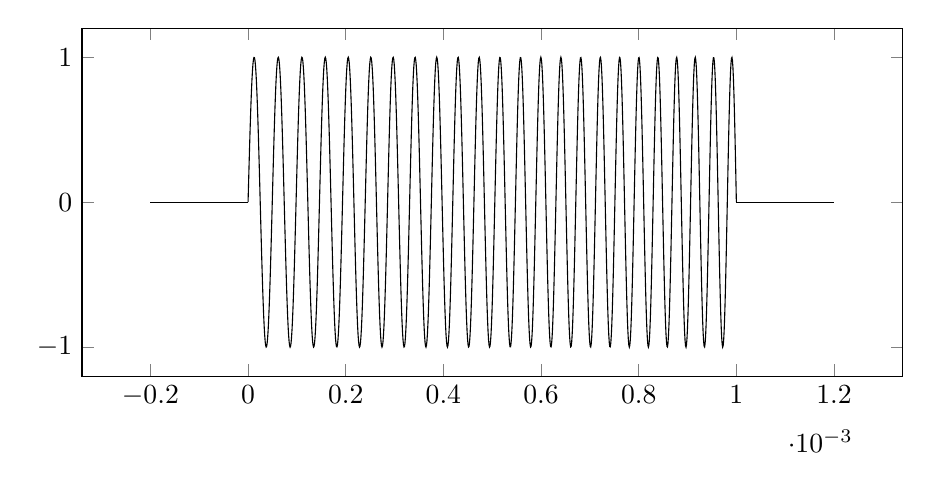
\begin{tikzpicture}
          \begin{axis}[width=12cm,height=6cm]
            \addplot[domain=-.0002:0,samples=10]{0};
            \addplot[domain=0:0.001,samples=1000]{sin((2*180*((27000 - 20000)/(2*0.001)*x*x + 20000*x)))};
            \addplot[domain=0.001:0.0012,samples=10]{0};
          \end{axis}
        \end{tikzpicture}
        \caption{Chirp signal with $\phi=0$, $A=1$, $f_0=\SI{20}{\kilo\hertz}$, $f_1=\SI{27}{\kilo\hertz}$, and $T=\SI{1}{\milli\second}$}
        \label{fig:chirp}
      \end{figure}

        This is the waveform we will be emitting from the ultrasonic sensors. The benefit is that it can be high power and still allow the receiver to determine precisely where in the waveform it is listening. One method for doing this is to take the discrete short time Fourier transform, which will show us how the power at various frequencies changes over time. By applying the FFT at a particular instant during the chirp, we can determine the position in time within the chirp of the current FFT. For instance, in the signal above if we apply and FFT at time $t_n=1.0$ and discover high power at frequency $f=\SI{22}{\kilo\hertz}$, we know that the chirp began at time $t_0 = t_n - \tfrac{f - f_0}{f_1 - f_0}T = 1.0 - \tfrac{22-20}{27-20}0.001 = 0.99857$. Another simpler strategy is to slide the waveform you expect to hear across samples of recorded raw input and check for the point of highest correlation. In other words, slide the waveform in Figure \ref{fig:chirp} and match it to the received signal. Both of these techniques are used in practice, and we are considering both in our implementation.

        Our beacon system relies on accurately knowing the distance to a beacon, and therefore knowing exactly when the start of the signal left the transmitter and when the start of the signal arrived at the receiver. Figure \ref{fig:rx_tx_timing} shows the sources of delay we are accounting for, and we describe our methodology for measuring these delays in the \nameref{section:experiments} section. \\

      \begin{figure}
        \centering
        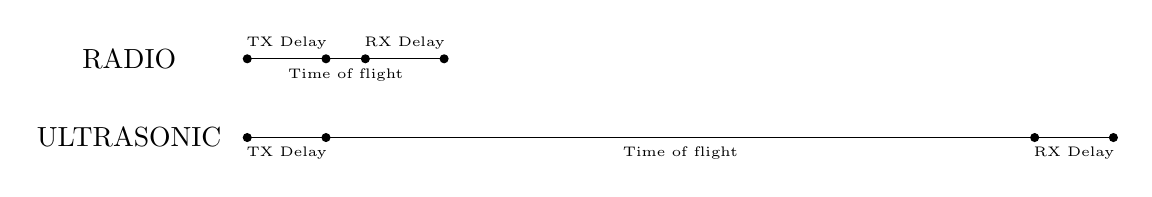
\begin{tikzpicture}
          % timeline for ultrasonic
          \draw (-1.5, 0) node {ULTRASONIC};
          \filldraw (0,0) circle (0.05);
          \draw (0.5, -0.2) node {\tiny TX Delay};
          \draw (0,0) -- (1,0);
          \filldraw (1,0) circle (0.05);
          \draw (5.5, -0.2) node {\tiny Time of flight};
          \draw (1,0) -- (10,0);
          \filldraw (10,0) circle (0.05);
          \draw (10.5, -0.2) node {\tiny RX Delay};
          \draw (10,0) -- (11,0);
          \filldraw (11,0) circle (0.05);

          % timeline for radio
          \draw (-1.5, 1) node {RADIO};
          \filldraw (0,1) circle (0.05);
          \draw (0.5, 1.2) node {\tiny TX Delay};
          \draw (0,1) -- (1,1);
          \filldraw (1,1) circle (0.05);
          \draw (1.25, 0.8) node {\tiny Time of flight};
          \draw (1,1) -- (1.5,1);
          \filldraw (1.5,1) circle (0.05);
          \draw (2.0, 1.2) node {\tiny RX Delay};
          \draw (1.5,1) -- (2.5,1);
          \filldraw (2.5,1) circle (0.05);
        \end{tikzpicture}
        \caption{Timing of radio and ultrasonic signals. Experiments indicate \SI{46.175}{\micro\second} total RF delay and \SI{1}{\milli\second} total ultrasonic delay.}
        \label{fig:rx_tx_timing}
      \end{figure}

      \textbf{Path Loss} \\
      We calculate the free space path loss (FSPL) of the radio signals at the farthest distance from the beacons. For this calculation, we assume the worst case where the beacon is on the other side of the length field, which is $\SI{16.5}{\meter}$ away. Over the more realistic distance of half the width of the field (\SI{5.6}{\meter}), the path loss is only \SI{40}{\decibel}. \\
      $$ \text{FSPL} = 20\log_{10}\Bigg(\frac{4\pi Rf^2}{c^2}\Bigg) = 20\log_{10}\Bigg(\frac{4\pi*16.5*\SI{433e6}{\hertz}}{\SI{3e8}{\meter\per\second}}\Bigg) = 49.521 $$

      \begin{table}
        \begin{tabular}{|l|l|}
          \hline
          Item & Cost per Beacon \\
          \hline
          PSoc 5LP & \$10.00 \\
          RF Tx/Rx Pair & \$1.68 \\
          piezo speaker & \$1.65 \\
          9v battery & \$1.19 \\
          battery connector & \$0.54 \\
          LCD display & \$3.90 (optional) \\
          resistors and capacitors & \$5.00 (estimate) \\
          prototyping board & \$5.00 (estimate) \\
          \hline
          Total & 28.96 \\
          \hline
        \end{tabular}
        \caption{estimated bill of material for beacons}
        \label{table:beacon_bom}
      \end{table}

      \textbf{Self-Localization of Beacons} \label{section:beacon_self_localization}

      Beacons that can automatically discover each other and their relative positions will tremendously improve the easy of setup for the beacon system. We believe this is possible, and in this section we describe a protocol for doing so.

      When the first beacon is turned on, it will listen for radio packets for a brief period of time to check if it is the first beacon to be turned on. If it hears nothing, it will assume it is the first beacon and assign itself ID 0. This beacon will be responsible for sending the synchronizing radio pulse as well as handle the distribution of IDs to the other beacons. At this point, beacon 0 will send packets advertising that ID 1 is available. When the next beacon is turned on, it will get the message that ID 1 is available, assign itself that ID, and respond with an ACK message confirming that ID 1 is now taken. Beacon 0 will then begin advertising that ID 2 is available. This process continues for N beacons. Once each beacon has its assigned ID number, beacon 0 will start organizing the self-localization of each beacon. First, beacon 0 will send a packet telling everyone that beacon 0 will transmit ultrasonic. All beacons other than beacon 0 will hear this and start a timer, and beacon 0 will itself transmit ultrasonic. Each beacon will receive this ultrasonic and compute its distance to beacon 0. After waiting a fixed period of time (such as \SI{50}{\milli\second}) for this process to complete, beacon 0 will send a packet telling everyone that beacon 1 will transmit ultrasonic. This process continues until every beacon has recorded its distance to every other beacon. At this point, beacon 0 will tell each beacon sequentially to report its distance calculations to beacon 0. Beacon 0 will then compute the location of every beacons by minimizing the least squares error in the system of equations defining the beacon locations. Finally, it will report the resulting positions to all the beacons. These communications can also be monitors from a laptop with an inexpensive USB software defined radio, such that the status and result of this process can be shown in a GUI and debugging information can be communicated.

      \textbf{Number of Beacons Needed}

      The number of beacons can be decided once the range and beam pattern of the beacons is known. To do this, a rigorous test that measures the sound level at various angles and distance will be performed. Once this is known, we can offer a tool or set of steps to determine how many beacons are needed and where beacons should be placed.

    \subsubsection{User Interface (GUI)}

      As mentioned above, one of our goals is to develop a GUI. This GUI will serve several functions, such as displaying the position of the robot on the field, showing debug information from each subsystem, and allowing students to input parameters about their robot and their practice space. For example, doing forward kinematics with the encoders requires that the position of each wheel and encoder is known. Additionally, the GUI could allow a visual interface for the students to say where and how their practice space maps to the imaginary FRC field.

\section{Conclusion} \label{section:conclusion}

\section{Future Work} \label{section:future_work}

\section{Acknowledgements}

  We thank our advisors, Bradley Miller and William Michalson for their guidance. We also thank our sponsors, AndyMark and Kauai Labs for their generous donation of hardware. We'd like to thank Scott Libert and Eric Peters for their advice. Finally, we give a special thank you to FRC Team 261 Gael Force, for letting us use their practice FRC field.


\bibliographystyle{plain}
\bibliography{phil-mqp}


\section{Appendices}

  \subsection{Survey Responses}\label{appendix:survey}

    \begin{figure}[H]
      \centering
      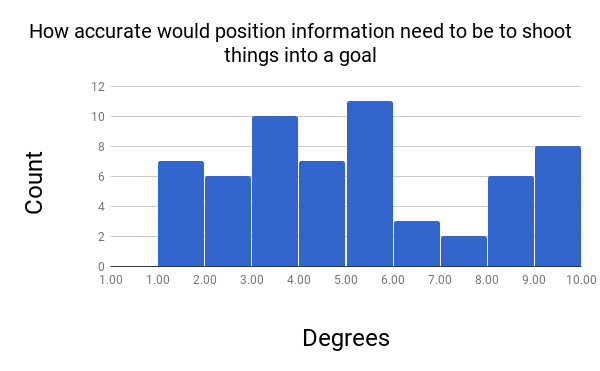
\includegraphics[height=4.2cm]{./images/survey_angle.png}
      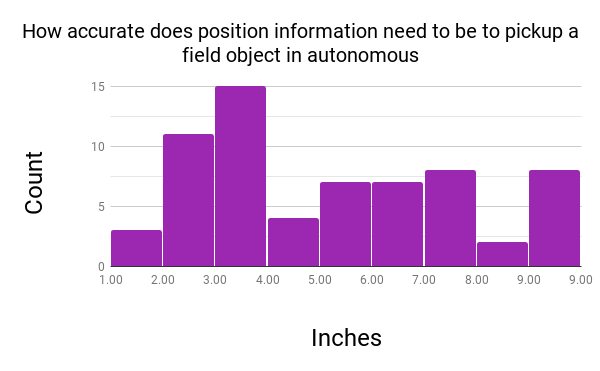
\includegraphics[height=4.2cm]{./images/survey_position.png}
      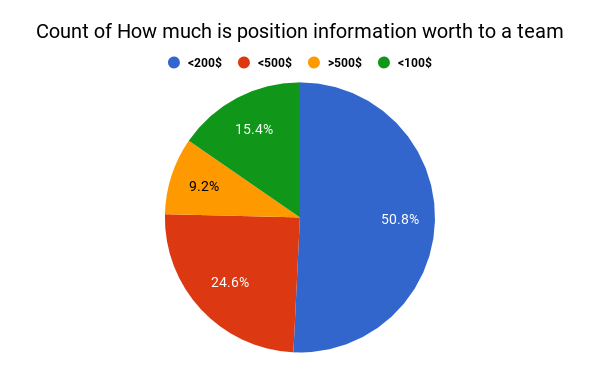
\includegraphics[height=4.2cm]{./images/survey_worth.png}
      \label{fig:survey_imgs}
    \end{figure}

  \subsection{Radio Time of Flight}\label{appendix:rf-rx-tx}

    \begin{table}[H]
      \begin{tabular}{|l|l|l|l|l|}
        \hline
        Measured Distance (m) & \multicolumn{3}{|l|}{Measured Total Time ($\mu$s)} & Average Delay \\
        \hline
        0.0630 & 45.44 & 42.80 & 34.48 & 40.90646 \\
        0.1425 & 52.72 & 50.48 & 52.09 & 51.76286 \\
        0.1505 & 64.16 & 63.36 & 60.24 & 62.58616 \\
        0.2210 & 40.33 & 36.79 & 36.40 & 37.83926 \\
        0.2415 & 49.52 & 45.76 & 43.92 & 46.39919 \\
        0.2460 & 47.47 & 53.84 & 44.71 & 48.67251 \\
        0.2965 & 34.36 & 34.00 & 43.76 & 37.37234 \\
        0.3085 & 79.36 & 62.16 & 59.52 & 67.01230 \\
        0.3390 & 39.92 & 57.27 & 38.96 & 45.38220 \\
        0.3770 & 41.75 & 40.75 & 45.53 & 42.67541 \\
        0.3600 & 38.40 & 38.40 & 37.68 & 38.15880 \\
        0.0070 & 35.60 & 36.08 & 34.32 & 35.33331 \\
        \hline
        \multicolumn{4}{|r|}{Average Delay ($\mu$s)} & 46.175 \\
        \hline
      \end{tabular}
      \caption{The time of flight of radio over tens of centimeters is insignificant compared to the delay within the transmitter and receiver.}
      \label{table:rf-rx-tx}
    \end{table}

  \subsection{ArUco Detection Times}\label{appendix:tag_detection}

    \begin{figure}[H]
      \centering
      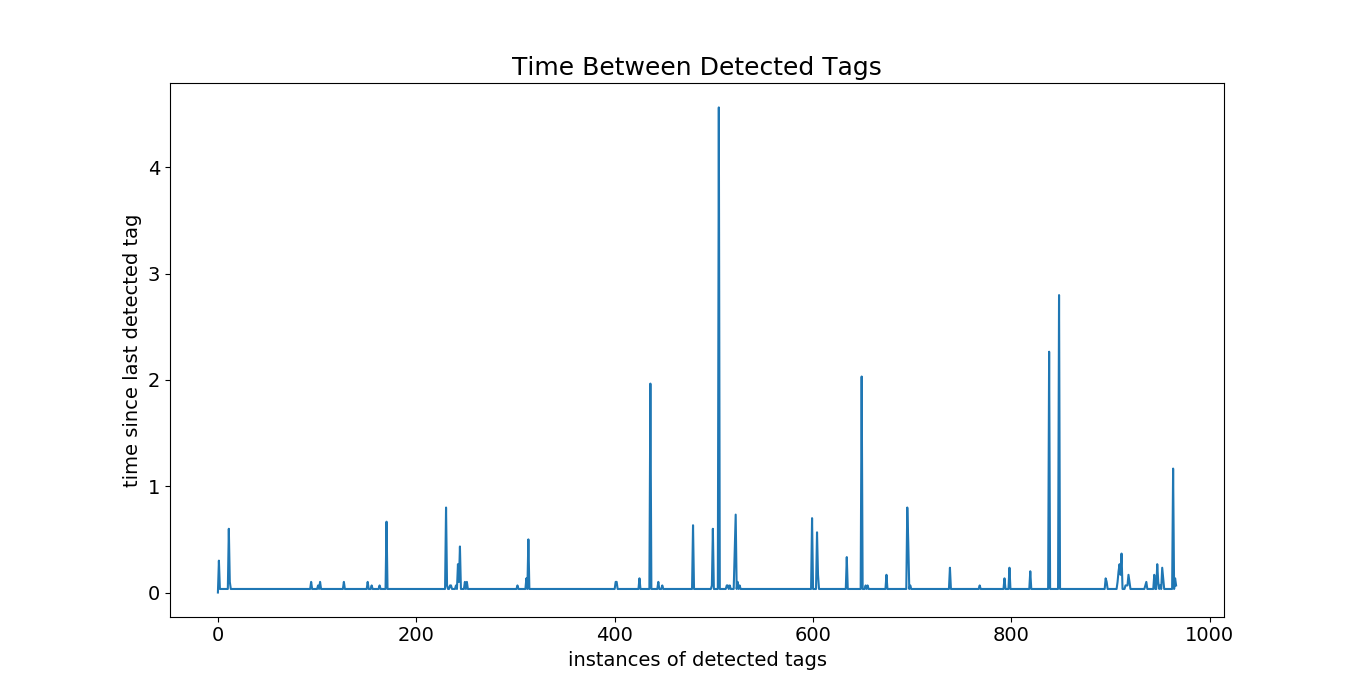
\includegraphics[width=1\linewidth]{./images/detection_times_480p30.png}
    \end{figure}
    \begin{figure}[H]
      \centering
      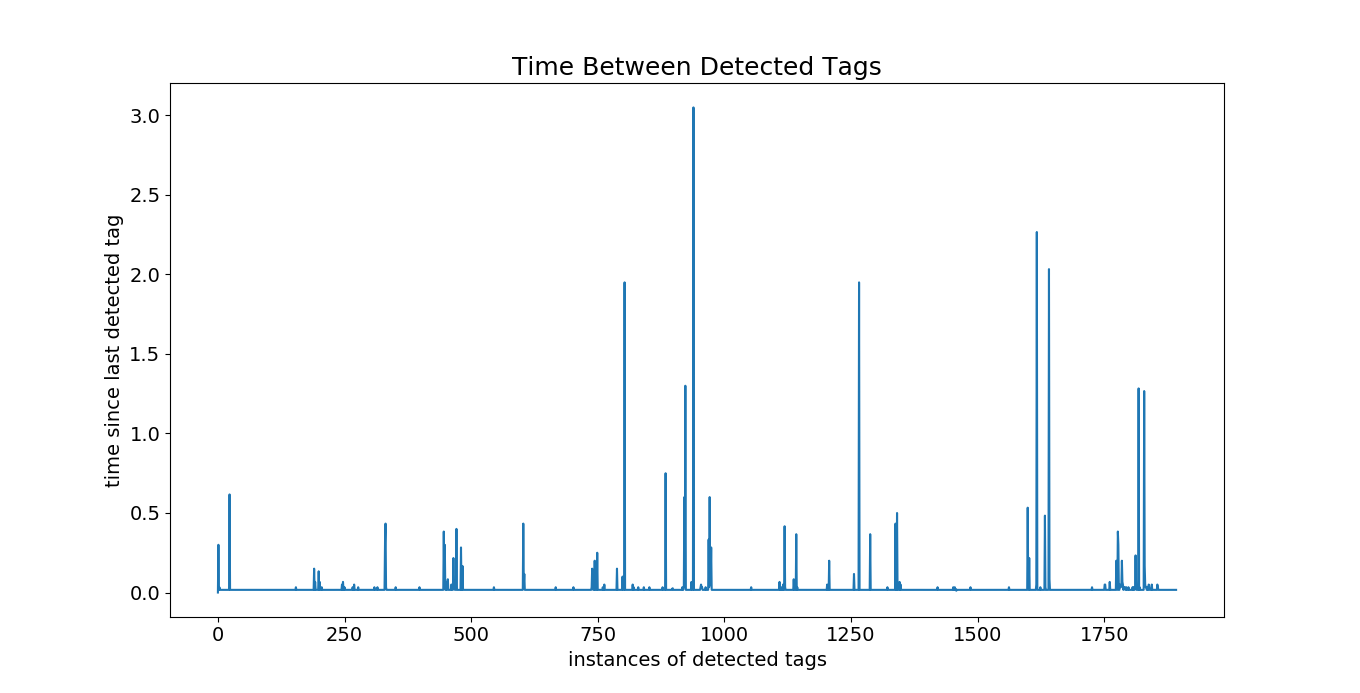
\includegraphics[width=1\linewidth]{./images/detection_times_480p60.png}
    \end{figure}
    \begin{figure}[H]
      \centering
      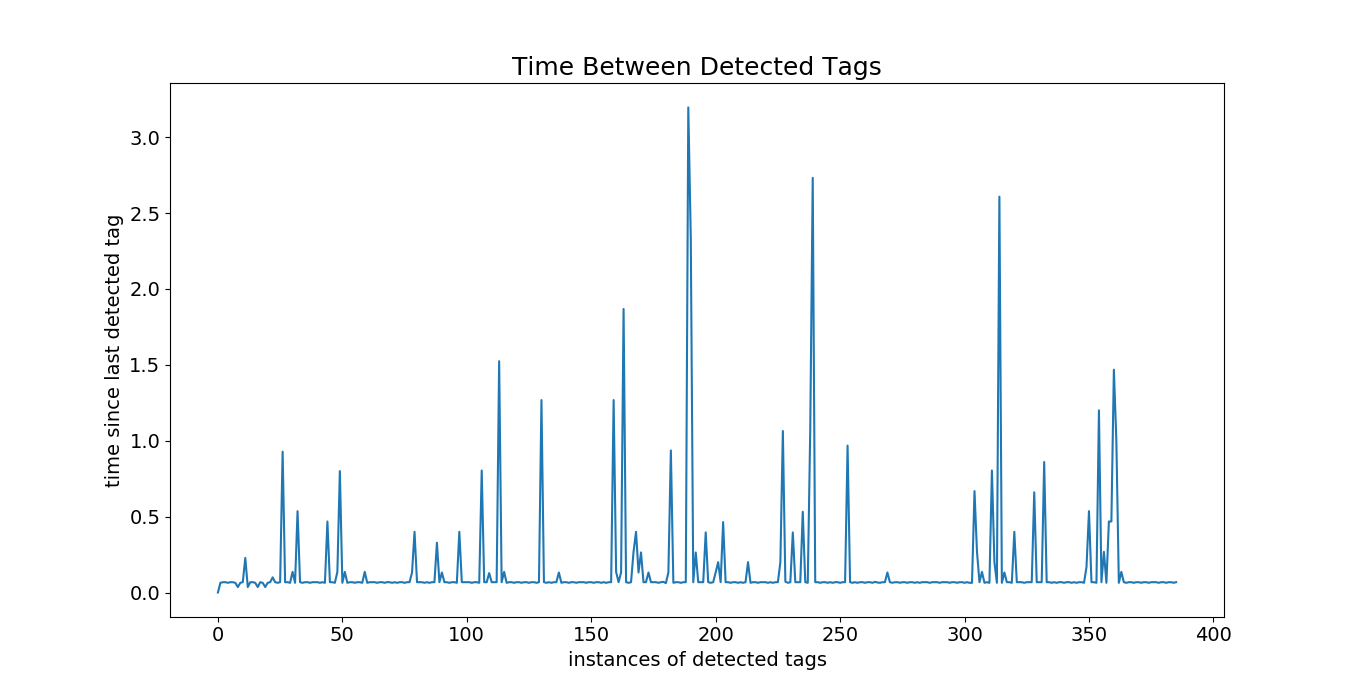
\includegraphics[width=1\linewidth]{./images/detection_times_1080p15.png}
    \end{figure}

  \subsection{Code \& Dataset}\label{appendix:code}

    All of the code used in the above experiments, including the sample implementation and all of the raw sensory data (minus large video files) are available in our github repository: \url{https://github.com/PHIL-MQP/phil}

\end{document}
